% ---------------------------------------------------------------------------- %
% file: dplyr_drug_talk.Rnw
% author: Peter DeWitt <peter.dewitt@ucdenver.edu>
%
% presentation on dplyr, and as a result also magrittr, for the Denver R User
% Group (DRUG) MeetUp on 1 July 2014.
%
% ---------------------------------------------------------------------------- %

\documentclass{beamer}\usepackage[]{graphicx}\usepackage[]{color}
%% maxwidth is the original width if it is less than linewidth
%% otherwise use linewidth (to make sure the graphics do not exceed the margin)
\makeatletter
\def\maxwidth{ %
  \ifdim\Gin@nat@width>\linewidth
    \linewidth
  \else
    \Gin@nat@width
  \fi
}
\makeatother

\definecolor{fgcolor}{rgb}{0.345, 0.345, 0.345}
\newcommand{\hlnum}[1]{\textcolor[rgb]{0.686,0.059,0.569}{#1}}%
\newcommand{\hlstr}[1]{\textcolor[rgb]{0.192,0.494,0.8}{#1}}%
\newcommand{\hlcom}[1]{\textcolor[rgb]{0.678,0.584,0.686}{\textit{#1}}}%
\newcommand{\hlopt}[1]{\textcolor[rgb]{0,0,0}{#1}}%
\newcommand{\hlstd}[1]{\textcolor[rgb]{0.345,0.345,0.345}{#1}}%
\newcommand{\hlkwa}[1]{\textcolor[rgb]{0.161,0.373,0.58}{\textbf{#1}}}%
\newcommand{\hlkwb}[1]{\textcolor[rgb]{0.69,0.353,0.396}{#1}}%
\newcommand{\hlkwc}[1]{\textcolor[rgb]{0.333,0.667,0.333}{#1}}%
\newcommand{\hlkwd}[1]{\textcolor[rgb]{0.737,0.353,0.396}{\textbf{#1}}}%

\usepackage{framed}
\makeatletter
\newenvironment{kframe}{%
 \def\at@end@of@kframe{}%
 \ifinner\ifhmode%
  \def\at@end@of@kframe{\end{minipage}}%
  \begin{minipage}{\columnwidth}%
 \fi\fi%
 \def\FrameCommand##1{\hskip\@totalleftmargin \hskip-\fboxsep
 \colorbox{shadecolor}{##1}\hskip-\fboxsep
     % There is no \\@totalrightmargin, so:
     \hskip-\linewidth \hskip-\@totalleftmargin \hskip\columnwidth}%
 \MakeFramed {\advance\hsize-\width
   \@totalleftmargin\z@ \linewidth\hsize
   \@setminipage}}%
 {\par\unskip\endMakeFramed%
 \at@end@of@kframe}
\makeatother

\definecolor{shadecolor}{rgb}{.97, .97, .97}
\definecolor{messagecolor}{rgb}{0, 0, 0}
\definecolor{warningcolor}{rgb}{1, 0, 1}
\definecolor{errorcolor}{rgb}{1, 0, 0}
\newenvironment{knitrout}{}{} % an empty environment to be redefined in TeX

\usepackage{alltt}

% preamble%{{{
\setbeamersize{text margin left=5pt,text margin right=5pt}
\usefonttheme{serif} 
\usepackage{verbatim}

\author{Peter DeWitt\\peter.dewitt@ucdenver.edu}
\date{1 July 2014}
\title{Introduction to {\tt dplyr} and {\tt magrittr}}
\subtitle{Denver R Users Group\\www.meetup.com/DenverRUG}


%}}}
\IfFileExists{upquote.sty}{\usepackage{upquote}}{}
\begin{document}

% Title page, goals%{{{
\begin{frame}[fragile]
  \maketitle
\end{frame} 

\begin{frame}[fragile]
  \frametitle{Goals:}

  \begin{itemize}
    \item Showcase {\tt dplyr}, compare the ease of use and speed to base R.
    \item Introduce the data manipulation grammar and philosophy behind {\tt
      dplyr}
    \item Illustrate the usefulness of the forward-piping operator which is
      part of {\tt dplyr} and extended further in {\tt magrittr}.  

    \item[]

    \item Convey: {\tt dplyr} will save time in initial coding, debugging, code
      maintenance, \ldots
  \end{itemize}

  % \tableofcontents

\end{frame} 

\begin{frame}[fragile]
  \frametitle{Is it Worth the Time?}
  \framesubtitle{\url{http://xkcd.com/1205/}}

  \begin{center}
    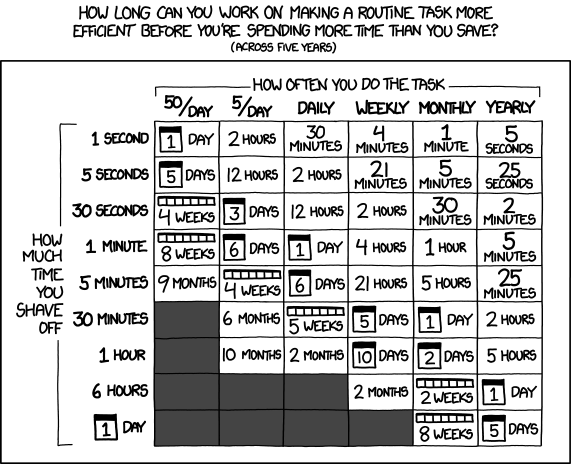
\includegraphics[width=0.75\textwidth]{../figure/is_it_worth_the_time} 
  \end{center}
\end{frame} 
%}}}

\section{{\tt dplyr}}%{{{
\begin{frame}[fragile]
  \frametitle{{\tt dplyr}: a grammar of data manipulation}
  \begin{itemize}
    \item Authored by Hadley Wickham and Romain Francois
    \item Current CRAN version 0.2

    \item<2-> Paraphrasing from a post on the RStudio blog
      \url{http://blog.rstudio.org/2014/01/17/introducing-dplyr}

      \begin{itemize}
        \item {\tt dplyr} is the next iteration of {\tt plyr}
        \item focuses only on {\tt data.frame}s
        \item faster, thanks in part to Francois work in {\tt Rcpp}, some use of
          multiple processors.
        \item improved API. 
        \item interface with remote database (PostgreSQL, MySQL, SQLite, and
          Google bigquery) tables using the same verbs for
          interacting with {\tt data.frame}s.  (Extendible to other backends)
        \item Common operations:
          \begin{itemize}
            \item {\tt group\_by}, {\tt summarize}, {\tt mutate}, {\tt filter},
              {\tt select}, and {\tt arrange}.
          \end{itemize}
      \end{itemize}

  \end{itemize}
\end{frame} 
%}}}

\subsection{Data Import}%{{{

\begin{frame}[fragile]
  \frametitle{Data Import}
  {\tt dplyr} does not have special tools for reading in data, but, if you need
  to {\tt rbind} sets together\ldots 



\begin{knitrout}\footnotesize
\definecolor{shadecolor}{rgb}{0.969, 0.969, 0.969}\color{fgcolor}\begin{kframe}
\begin{alltt}
\hlcom{# FAAs wildlife strikes on aircraft since 1990.  The data}
\hlcom{# can be downloaded, in a Microsoft Access DB,  from}
\hlcom{# http://www.faa.gov/airports/airport_safety/wildlife/database/}
\hlcom{# Tables in the DB were exported to csv files.  }
\hlcom{# A data dictionary, in an Excel file, was also}
\hlcom{# included in the download from faa.gov}

\hlcom{# column classes are set (in R code not shown) to ensure}
\hlcom{# that each column of the imported data is of the same class}
\hlstd{wls.90.99} \hlkwb{<-} \hlkwd{read.csv}\hlstd{(}\hlstr{"../data/STRIKE_REPORTS (1990-1999).csv"}\hlstd{,}
                      \hlkwc{colClasses} \hlstd{= clclss)}
\hlstd{wls.00.09} \hlkwb{<-} \hlkwd{read.csv}\hlstd{(}\hlstr{"../data/STRIKE_REPORTS (2000-2009).csv"}\hlstd{,}
                      \hlkwc{colClasses} \hlstd{= clclss)}
\hlstd{wls.10.14} \hlkwb{<-} \hlkwd{read.csv}\hlstd{(}\hlstr{"../data/STRIKE_REPORTS (2010-Current).csv"}\hlstd{,}
                      \hlkwc{colClasses} \hlstd{= clclss)}
\end{alltt}
\end{kframe}
\end{knitrout}
\end{frame} 


\begin{frame}[fragile]
  \frametitle{Data Import}
\begin{knitrout}\footnotesize
\definecolor{shadecolor}{rgb}{0.969, 0.969, 0.969}\color{fgcolor}\begin{kframe}
\begin{alltt}
\hlkwd{dim}\hlstd{(wls.90.99)}
\end{alltt}
\begin{verbatim}
## [1] 30150    94
\end{verbatim}
\begin{alltt}
\hlkwd{nrow}\hlstd{(wls.90.99)} \hlopt{+} \hlkwd{nrow}\hlstd{(wls.00.09)} \hlopt{+} \hlkwd{nrow}\hlstd{(wls.10.14)}
\end{alltt}
\begin{verbatim}
## [1] 142911
\end{verbatim}
\begin{alltt}
\hlstd{bnchmrk} \hlkwb{<-}
  \hlkwd{benchmark}\hlstd{(}\hlkwc{base}  \hlstd{=} \hlkwd{rbind}\hlstd{(wls.90.99, wls.00.09, wls.10.14),}
            \hlkwc{dplyr} \hlstd{=} \hlkwd{rbind_list}\hlstd{(wls.90.99, wls.00.09, wls.10.14),}
            \hlkwc{replications} \hlstd{=} \hlnum{100}\hlstd{)}
\hlstd{bnchmrk[,} \hlkwd{c}\hlstd{(}\hlstr{"test"}\hlstd{,} \hlstr{"replications"}\hlstd{,} \hlstr{"elapsed"}\hlstd{,} \hlstr{"relative"}\hlstd{)]}
\end{alltt}
\begin{verbatim}
##    test replications elapsed relative
## 1  base          100   48.43    4.017
## 2 dplyr          100   12.05    1.000
\end{verbatim}
\end{kframe}
\end{knitrout}
\end{frame} 

\begin{frame}[fragile]
  \frametitle{Data Import}
\begin{knitrout}\footnotesize
\definecolor{shadecolor}{rgb}{0.969, 0.969, 0.969}\color{fgcolor}\begin{kframe}
\begin{alltt}
\hlstd{wls_df} \hlkwb{<-} \hlkwd{rbind}\hlstd{(wls.90.99, wls.00.09, wls.10.14)}
\hlkwd{class}\hlstd{(wls_df)}
\end{alltt}
\begin{verbatim}
## [1] "data.frame"
\end{verbatim}
\begin{alltt}
\hlstd{wls} \hlkwb{<-} \hlkwd{rbind_list}\hlstd{(wls.90.99, wls.00.09, wls.10.14)}
\hlkwd{class}\hlstd{(wls)}
\end{alltt}
\begin{verbatim}
## [1] "data.frame"
\end{verbatim}
\begin{alltt}
\hlcom{# A data frame tbl wraps a local data frame. The main}
\hlcom{# advantage to using a ‘tbl_df’ over a regular data frame is}
\hlcom{# the printing: tbl objects only print a few rows and all}
\hlcom{# the columns that fit on one screen, providing describing}
\hlcom{# the rest of it as text. [source: R help doc]}
\hlstd{wls_tbl_df} \hlkwb{<-} \hlkwd{tbl_df}\hlstd{(wls)}
\hlkwd{class}\hlstd{(wls_tbl_df)}
\end{alltt}
\begin{verbatim}
## [1] "tbl_df"     "tbl"        "data.frame"
\end{verbatim}
\end{kframe}
\end{knitrout}
\end{frame} 

\begin{frame}[fragile]
  \frametitle{Data Printing}
\begin{knitrout}\footnotesize
\definecolor{shadecolor}{rgb}{0.969, 0.969, 0.969}\color{fgcolor}\begin{kframe}
\begin{alltt}
\hlcom{# print(wls_df)  # takes a long time, not helpful}
\hlcom{# head(wls_df)   # too many columns to be useful}
\hlkwd{print}\hlstd{(wls_tbl_df,} \hlkwc{n} \hlstd{=} \hlnum{3}\hlstd{)}
\end{alltt}
\begin{verbatim}
## Source: local data frame [142,911 x 94]
## 
##    INDEX_NR OPID          OPERATOR     ATYPE AMA AMO EMA EMO
## 1    100000  AAL AMERICAN AIRLINES     B-727 148  10  34  10
## 2    100001  UAL   UNITED AIRLINES B-737-300 148  24  10  01
## 3    100002  UAL   UNITED AIRLINES B-737-300 148  24  10  01
## ..      ...  ...               ...       ... ... ... ... ...
## Variables not shown: AC_CLASS (chr), AC_MASS (int), NUM_ENGS
##   (chr), TYPE_ENG (chr), ENG_1_POS (chr), ENG_2_POS (int),
##   ENG_3_POS (chr), ENG_4_POS (int), REG (chr), FLT (chr),
##   REMAINS_COLLECTED (lgl), REMAINS_SENT (lgl), INCIDENT_DATE
##   (chr), INCIDENT_MONTH (int), INCIDENT_YEAR (int),
##   TIME_OF_DAY (chr), TIME (int), AIRPORT_ID (chr), AIRPORT
##   (chr), STATE (chr), FAAREGION (chr), ENROUTE (chr), RUNWAY
##   (chr), LOCATION (chr), HEIGHT (int), SPEED (int), DISTANCE
##   (dbl), PHASE_OF_FLT (chr), DAMAGE (chr), STR_RAD (lgl),
##   DAM_RAD (lgl), STR_WINDSHLD (lgl), DAM_WINDSHLD (lgl),
##   STR_NOSE (lgl), DAM_NOSE (lgl), STR_ENG1 (lgl), DAM_ENG1
##   (lgl), STR_ENG2 (lgl), DAM_ENG2 (lgl), STR_ENG3 (lgl),
##   DAM_ENG3 (lgl), STR_ENG4 (lgl), DAM_ENG4 (lgl), INGESTED
##   (lgl), STR_PROP (lgl), DAM_PROP (lgl), STR_WING_ROT (lgl),
##   DAM_WING_ROT (lgl), STR_FUSE (lgl), DAM_FUSE (lgl), STR_LG
##   (lgl), DAM_LG (lgl), STR_TAIL (lgl), DAM_TAIL (lgl),
##   STR_LGHTS (lgl), DAM_LGHTS (lgl), STR_OTHER (lgl),
##   DAM_OTHER (lgl), OTHER_SPECIFY (chr), EFFECT (chr),
##   EFFECT_OTHER (chr), SKY (chr), PRECIP (chr), SPECIES_ID
##   (chr), SPECIES (chr), BIRDS_SEEN (chr), BIRDS_STRUCK (chr),
##   SIZE (chr), WARNED (chr), COMMENTS (chr), REMARKS (chr),
##   AOS (int), COST_REPAIRS (int), COST_OTHER (int),
##   COST_REPAIRS_INFL_ADJ (int), COST_OTHER_INFL_ADJ (int),
##   REPORTED_NAME (chr), REPORTED_TITLE (chr), REPORTED_DATE
##   (chr), SOURCE (chr), PERSON (chr), NR_INJURIES (int),
##   NR_FATALITIES (int), LUPDATE (chr), TRANSFER (lgl),
##   INDICATED_DAMAGE (lgl)
\end{verbatim}
\end{kframe}
\end{knitrout}
\end{frame} 
%}}}

\subsection{{\tt dplyr} verbs}%{{{
\begin{frame}[fragile]
  \frametitle{The verbs}
  \begin{itemize}
    \item ``Variable and function names should be lowercase. Use an underscore
      (\_) to separate words within a name. Generally, variable names should be
      nouns and function names should be verbs. Strive for names that are
      concise and meaningful (this is not easy!).'' - Hadley Wickham,
      \url{http://adv-r.had.co.nz/Style.html}

    \item[]

    \item Verbs in {\tt dplyr} 
      \begin{itemize}
        \item {\tt select},
        \item {\tt arrange},
        \item {\tt filter},
        \item {\tt mutate}, 
        \item {\tt summarize}.
      \end{itemize}
  \end{itemize}
\end{frame} 
%}}}

\subsubsection{select}%{{{

\begin{frame}[fragile]
  \frametitle{{\tt select}}
\begin{knitrout}\footnotesize
\definecolor{shadecolor}{rgb}{0.969, 0.969, 0.969}\color{fgcolor}\begin{kframe}
\begin{alltt}
\hlcom{# Select columns of a data.frame, tbl_df.}
\hlstd{wls_yr} \hlkwb{<-} \hlkwd{select}\hlstd{(wls_tbl_df, INCIDENT_YEAR, AIRPORT,}
                 \hlstd{ENG_1_POS, ENG_2_POS, DAM_ENG1, DAM_ENG2,}
                 \hlstd{HEIGHT, DISTANCE, SPEED)}
\hlkwd{print}\hlstd{(wls_yr,} \hlkwc{n} \hlstd{=} \hlnum{5}\hlstd{)}
\end{alltt}
\begin{verbatim}
## Source: local data frame [142,911 x 9]
## 
##    INCIDENT_YEAR                     AIRPORT ENG_1_POS
## 1           1992 DALLAS/FORT WORTH INTL ARPT         5
## 2           1996             SACRAMENTO INTL         1
## 3           1996         DENVER INTL AIRPORT         1
## 4           1996             EPPLEY AIRFIELD         1
## 5           1996 WASHINGTON DULLES INTL ARPT         1
## ..           ...                         ...       ...
## Variables not shown: ENG_2_POS (int), DAM_ENG1 (lgl),
##   DAM_ENG2 (lgl), HEIGHT (int), DISTANCE (dbl), SPEED (int)
\end{verbatim}
\end{kframe}
\end{knitrout}
\end{frame} 

\begin{frame}[fragile]
  \frametitle{{\tt select}}
\begin{knitrout}\footnotesize
\definecolor{shadecolor}{rgb}{0.969, 0.969, 0.969}\color{fgcolor}\begin{kframe}
\begin{alltt}
\hlcom{# relative speed betwwen dplyr and base R}
\hlstd{bnch} \hlkwb{<-}
  \hlkwd{benchmark}\hlstd{(}\hlkwc{base}  \hlstd{= wls_tbl_df[,} \hlkwd{c}\hlstd{(}\hlstr{"INCIDENT_YEAR"}\hlstd{,} \hlstr{"AIRPORT"}\hlstd{,}
                                   \hlstr{"ENG_1_POS"}\hlstd{,} \hlstr{"ENG_2_POS"}\hlstd{,}
                                   \hlstr{"DAM_ENG1"}\hlstd{,} \hlstr{"DAM_ENG2"}\hlstd{,}
                                   \hlstr{"HEIGHT"}\hlstd{,} \hlstr{"DISTANCE"}\hlstd{,} \hlstr{"SPEED"}\hlstd{)],}
            \hlkwc{dplyr} \hlstd{=} \hlkwd{select}\hlstd{(wls_tbl_df,}
                           \hlstd{INCIDENT_YEAR, AIRPORT,}
                           \hlstd{ENG_1_POS, ENG_2_POS,}
                           \hlstd{DAM_ENG1, DAM_ENG2,}
                           \hlstd{HEIGHT, DISTANCE, SPEED),}
            \hlkwc{replications} \hlstd{=} \hlnum{100}\hlstd{)}
\hlkwd{select}\hlstd{(bnch, test, replications, elapsed, relative)}
\end{alltt}
\begin{verbatim}
##    test replications elapsed relative
## 1  base          100   0.003    1.000
## 2 dplyr          100   0.013    4.333
\end{verbatim}
\end{kframe}
\end{knitrout}

Selection of columns might be slower in dplyr, but, there are some
tools to help speed up the coding, and maintenance.  {\tt select} will be very
helpful when chaining together many operations or when using \emph{super cool
helper functions}.
\end{frame} 


\begin{frame}[fragile]
  \frametitle{{\tt select}}
\begin{knitrout}\footnotesize
\definecolor{shadecolor}{rgb}{0.969, 0.969, 0.969}\color{fgcolor}\begin{kframe}
\begin{alltt}
\hlcom{# ‘num_range("x", 1:5, width = 2)’: selects all variables}
\hlcom{# (numerically) from x01 to x05.}
\hlkwd{select}\hlstd{(wls_tbl_df,} \hlkwd{num_range}\hlstd{(}\hlstr{"DAM_ENG"}\hlstd{,} \hlnum{1}\hlopt{:}\hlnum{4}\hlstd{))}
\end{alltt}
\begin{verbatim}
## Source: local data frame [142,911 x 4]
## 
##    DAM_ENG1 DAM_ENG2 DAM_ENG3 DAM_ENG4
## 1     FALSE    FALSE    FALSE    FALSE
## 2     FALSE    FALSE    FALSE    FALSE
## 3     FALSE    FALSE    FALSE    FALSE
## 4     FALSE    FALSE    FALSE    FALSE
## 5     FALSE    FALSE    FALSE    FALSE
## 6     FALSE    FALSE    FALSE    FALSE
## 7     FALSE    FALSE    FALSE    FALSE
## 8     FALSE    FALSE    FALSE    FALSE
## 9     FALSE    FALSE    FALSE    FALSE
## 10    FALSE    FALSE    FALSE    FALSE
## ..      ...      ...      ...      ...
\end{verbatim}
\end{kframe}
\end{knitrout}
\end{frame} 

\begin{frame}[fragile]
  \frametitle{{\tt select}}
\begin{knitrout}\footnotesize
\definecolor{shadecolor}{rgb}{0.969, 0.969, 0.969}\color{fgcolor}\begin{kframe}
\begin{alltt}
\hlcom{# ‘starts_with(x, ignore.case = FALSE)’: names starts with ‘x’}
\hlkwd{select}\hlstd{(wls_tbl_df,} \hlkwd{starts_with}\hlstd{(}\hlstr{"DAM"}\hlstd{))}
\end{alltt}
\begin{verbatim}
## Source: local data frame [142,911 x 15]
## 
##    DAMAGE DAM_RAD DAM_WINDSHLD DAM_NOSE DAM_ENG1 DAM_ENG2
## 1       N   FALSE        FALSE    FALSE    FALSE    FALSE
## 2           FALSE        FALSE    FALSE    FALSE    FALSE
## 3           FALSE        FALSE    FALSE    FALSE    FALSE
## 4       N   FALSE        FALSE    FALSE    FALSE    FALSE
## 5       N   FALSE        FALSE    FALSE    FALSE    FALSE
## 6       M   FALSE        FALSE    FALSE    FALSE    FALSE
## 7       N   FALSE        FALSE    FALSE    FALSE    FALSE
## 8      M?   FALSE        FALSE    FALSE    FALSE    FALSE
## 9       N   FALSE        FALSE    FALSE    FALSE    FALSE
## 10          FALSE        FALSE    FALSE    FALSE    FALSE
## ..    ...     ...          ...      ...      ...      ...
## Variables not shown: DAM_ENG3 (lgl), DAM_ENG4 (lgl), DAM_PROP
##   (lgl), DAM_WING_ROT (lgl), DAM_FUSE (lgl), DAM_LG (lgl),
##   DAM_TAIL (lgl), DAM_LGHTS (lgl), DAM_OTHER (lgl)
\end{verbatim}
\end{kframe}
\end{knitrout}
\end{frame} 

\begin{frame}[fragile]
  \frametitle{{\tt select}}
\begin{knitrout}\footnotesize
\definecolor{shadecolor}{rgb}{0.969, 0.969, 0.969}\color{fgcolor}\begin{kframe}
\begin{alltt}
\hlcom{# ‘ends_with(x, ignore.case = FALSE)’: names ends in ‘x’}
\hlkwd{select}\hlstd{(wls_tbl_df,} \hlkwd{ends_with}\hlstd{(}\hlstr{"4"}\hlstd{))}
\end{alltt}
\begin{verbatim}
## Source: local data frame [142,911 x 2]
## 
##    STR_ENG4 DAM_ENG4
## 1     FALSE    FALSE
## 2     FALSE    FALSE
## 3     FALSE    FALSE
## 4     FALSE    FALSE
## 5     FALSE    FALSE
## 6     FALSE    FALSE
## 7     FALSE    FALSE
## 8     FALSE    FALSE
## 9     FALSE    FALSE
## 10    FALSE    FALSE
## ..      ...      ...
\end{verbatim}
\end{kframe}
\end{knitrout}
\end{frame} 

\begin{frame}[fragile]
  \frametitle{{\tt select}}
\begin{knitrout}\footnotesize
\definecolor{shadecolor}{rgb}{0.969, 0.969, 0.969}\color{fgcolor}\begin{kframe}
\begin{alltt}
\hlcom{# ‘matches(x, ignore.case = FALSE)’: selects all variables}
\hlcom{# whose name matches the regular expression ‘x’}
\hlkwd{select}\hlstd{(wls_tbl_df,} \hlkwd{matches}\hlstd{(}\hlstr{"ENG|DAM"}\hlstd{))}
\end{alltt}
\begin{verbatim}
## Source: local data frame [142,911 x 26]
## 
##    NUM_ENGS TYPE_ENG ENG_1_POS ENG_2_POS ENG_3_POS ENG_4_POS
## 1         3        D         5         6         5        NA
## 2         2        D         1         1                  NA
## 3         2        D         1         1                  NA
## 4         2        D         1         1                  NA
## 5         2        D         1         1                  NA
## 6         2        D         1         1                  NA
## 7         3        D         5         6         5        NA
## 8         2        C         4         4                  NA
## 9         2        D         1         1                  NA
## 10        2        D         5         5                  NA
## ..      ...      ...       ...       ...       ...       ...
## Variables not shown: DAMAGE (chr), DAM_RAD (lgl),
##   DAM_WINDSHLD (lgl), DAM_NOSE (lgl), STR_ENG1 (lgl),
##   DAM_ENG1 (lgl), STR_ENG2 (lgl), DAM_ENG2 (lgl), STR_ENG3
##   (lgl), DAM_ENG3 (lgl), STR_ENG4 (lgl), DAM_ENG4 (lgl),
##   DAM_PROP (lgl), DAM_WING_ROT (lgl), DAM_FUSE (lgl), DAM_LG
##   (lgl), DAM_TAIL (lgl), DAM_LGHTS (lgl), DAM_OTHER (lgl),
##   INDICATED_DAMAGE (lgl)
\end{verbatim}
\end{kframe}
\end{knitrout}
\end{frame} 

\begin{frame}[fragile]
  \frametitle{{\tt select}}
\begin{knitrout}\footnotesize
\definecolor{shadecolor}{rgb}{0.969, 0.969, 0.969}\color{fgcolor}\begin{kframe}
\begin{alltt}
\hlcom{# ‘contains(x, ignore.case = FALSE)’: selects all}
\hlcom{# variables whose name  contains ‘x’}
\hlkwd{select}\hlstd{(wls_tbl_df,} \hlkwd{contains}\hlstd{(}\hlstr{"ENG"}\hlstd{))}
\end{alltt}
\begin{verbatim}
## Source: local data frame [142,911 x 14]
## 
##    NUM_ENGS TYPE_ENG ENG_1_POS ENG_2_POS ENG_3_POS ENG_4_POS
## 1         3        D         5         6         5        NA
## 2         2        D         1         1                  NA
## 3         2        D         1         1                  NA
## 4         2        D         1         1                  NA
## 5         2        D         1         1                  NA
## 6         2        D         1         1                  NA
## 7         3        D         5         6         5        NA
## 8         2        C         4         4                  NA
## 9         2        D         1         1                  NA
## 10        2        D         5         5                  NA
## ..      ...      ...       ...       ...       ...       ...
## Variables not shown: STR_ENG1 (lgl), DAM_ENG1 (lgl), STR_ENG2
##   (lgl), DAM_ENG2 (lgl), STR_ENG3 (lgl), DAM_ENG3 (lgl),
##   STR_ENG4 (lgl), DAM_ENG4 (lgl)
\end{verbatim}
\end{kframe}
\end{knitrout}
\end{frame} 

\begin{frame}[fragile]
  \frametitle{{\tt select}}
  What about dropping variables?
\begin{knitrout}\footnotesize
\definecolor{shadecolor}{rgb}{0.969, 0.969, 0.969}\color{fgcolor}\begin{kframe}
\begin{alltt}
\hlkwd{print}\hlstd{(wls_yr,} \hlkwc{n} \hlstd{=} \hlnum{2}\hlstd{)}
\end{alltt}
\begin{verbatim}
## Source: local data frame [142,911 x 9]
## 
##    INCIDENT_YEAR                     AIRPORT ENG_1_POS
## 1           1992 DALLAS/FORT WORTH INTL ARPT         5
## 2           1996             SACRAMENTO INTL         1
## ..           ...                         ...       ...
## Variables not shown: ENG_2_POS (int), DAM_ENG1 (lgl),
##   DAM_ENG2 (lgl), HEIGHT (int), DISTANCE (dbl), SPEED (int)
\end{verbatim}
\begin{alltt}
\hlcom{# omit AIRPORT and any column with a name starting with ENG.}
\hlkwd{print}\hlstd{(}\hlkwd{select}\hlstd{(wls_yr,} \hlopt{-}\hlstd{AIRPORT,} \hlopt{-}\hlkwd{starts_with}\hlstd{(}\hlstr{"ENG"}\hlstd{)),} \hlkwc{n} \hlstd{=} \hlnum{3}\hlstd{)}
\end{alltt}
\begin{verbatim}
## Source: local data frame [142,911 x 6]
## 
##    INCIDENT_YEAR DAM_ENG1 DAM_ENG2 HEIGHT DISTANCE SPEED
## 1           1992    FALSE    FALSE    300       NA   142
## 2           1996    FALSE    FALSE      0        0    NA
## 3           1996    FALSE    FALSE      0        0    NA
## ..           ...      ...      ...    ...      ...   ...
\end{verbatim}
\end{kframe}
\end{knitrout}
\end{frame} 
%}}}

\subsubsection{arrange}%{{{

\begin{frame}[fragile]
  \frametitle{{\tt arrange}}
arrange: reorder the rows. Multiple inputs are ordered from left-to-right.
\begin{knitrout}\footnotesize
\definecolor{shadecolor}{rgb}{0.969, 0.969, 0.969}\color{fgcolor}\begin{kframe}
\begin{alltt}
\hlstd{dat} \hlkwb{<-} \hlkwd{data.frame}\hlstd{(}\hlkwc{var1} \hlstd{=} \hlkwd{c}\hlstd{(}\hlnum{3}\hlstd{,} \hlnum{8}\hlstd{,} \hlnum{2}\hlstd{,} \hlnum{1}\hlstd{),}
                  \hlkwc{var2} \hlstd{=} \hlkwd{c}\hlstd{(}\hlstr{"E"}\hlstd{,} \hlstr{"A"}\hlstd{,} \hlstr{"A"}\hlstd{,} \hlstr{"B"}\hlstd{))}
\hlstd{dat}
\end{alltt}
\begin{verbatim}
##   var1 var2
## 1    3    E
## 2    8    A
## 3    2    A
## 4    1    B
\end{verbatim}
\end{kframe}
\end{knitrout}
\end{frame} 

\begin{frame}[fragile]
  \frametitle{{\tt arrange}}
\begin{knitrout}\footnotesize
\definecolor{shadecolor}{rgb}{0.969, 0.969, 0.969}\color{fgcolor}\begin{kframe}
\begin{alltt}
\hlkwd{arrange}\hlstd{(dat, var2)}
\end{alltt}
\begin{verbatim}
##   var1 var2
## 1    8    A
## 2    2    A
## 3    1    B
## 4    3    E
\end{verbatim}
\begin{alltt}
\hlkwd{arrange}\hlstd{(dat, var2, var1)}
\end{alltt}
\begin{verbatim}
##   var1 var2
## 1    2    A
## 2    8    A
## 3    1    B
## 4    3    E
\end{verbatim}
\begin{alltt}
\hlcom{# this would be very helpful for collecting data by a}
\hlcom{# subject id, visit number, ...}
\hlcom{#}
\hlcom{# Very helpful for geepack::geeglm() where the data *must* }
\hlcom{# be sorted by cluster and in temporal order as well.}
\end{alltt}
\end{kframe}
\end{knitrout}
\end{frame} 
%}}}

\subsubsection{filter}%{{{
\begin{frame}[fragile]
  \frametitle{{\tt filter}}
filter: return only a subset of the rows. If multiple
conditions are supplied they are combined with ‘\&’.
\begin{knitrout}\footnotesize
\definecolor{shadecolor}{rgb}{0.969, 0.969, 0.969}\color{fgcolor}\begin{kframe}
\begin{alltt}
\hlkwd{dim}\hlstd{(wls_yr)}
\end{alltt}
\begin{verbatim}
## [1] 142911      9
\end{verbatim}
\begin{alltt}
\hlkwd{filter}\hlstd{(wls_yr, INCIDENT_YEAR} \hlopt{>} \hlnum{2000}\hlstd{, INCIDENT_YEAR} \hlopt{<=} \hlnum{2005}\hlstd{)}
\end{alltt}
\begin{verbatim}
## Source: local data frame [31,947 x 9]
## 
##    INCIDENT_YEAR                       AIRPORT ENG_1_POS
## 1           2001           JOHN F KENNEDY INTL          
## 2           2001       SAN FRANCISCO INTL ARPT         1
## 3           2001                  ORLANDO INTL         1
## 4           2001                  MOLOKAI ARPT         4
## 5           2001         LAMBERT-ST LOUIS INTL         5
## 6           2001              KANSAS CITY INTL         1
## 7           2001                       UNKNOWN         1
## 8           2001         AKRON-CANTON REGIONAL         7
## 9           2001 DESTIN-FORT WALTON BEACH ARPT         5
## 10          2001           JOHN F KENNEDY INTL         1
## ..           ...                           ...       ...
## Variables not shown: ENG_2_POS (int), DAM_ENG1 (lgl),
##   DAM_ENG2 (lgl), HEIGHT (int), DISTANCE (dbl), SPEED (int)
\end{verbatim}
\end{kframe}
\end{knitrout}
\end{frame} 

\begin{frame}[fragile]
  \frametitle{{\tt filter}}

\begin{knitrout}\footnotesize
\definecolor{shadecolor}{rgb}{0.969, 0.969, 0.969}\color{fgcolor}\begin{kframe}
\begin{alltt}
\hlcom{# How does dplyr::filter compare to base::subset?}
\hlstd{bnch} \hlkwb{<-}
  \hlkwd{benchmark}\hlstd{(}\hlkwc{base} \hlstd{=} \hlkwd{subset}\hlstd{(wls_yr,}
                          \hlstd{INCIDENT_YEAR} \hlopt{>} \hlnum{2000} \hlopt{&} \hlstd{INCIDENT_YEAR} \hlopt{<=} \hlnum{2005}\hlstd{),}
            \hlkwc{dplyr} \hlstd{=} \hlkwd{filter}\hlstd{(wls_yr,}
                           \hlstd{INCIDENT_YEAR} \hlopt{>} \hlnum{2000}\hlstd{, INCIDENT_YEAR} \hlopt{<=} \hlnum{2005}\hlstd{),}
            \hlkwc{replications} \hlstd{=} \hlnum{100}\hlstd{)}
\hlkwd{select}\hlstd{(bnch, test, replications, elapsed, relative)}
\end{alltt}
\begin{verbatim}
##    test replications elapsed relative
## 1  base          100   3.607     5.25
## 2 dplyr          100   0.687     1.00
\end{verbatim}
\end{kframe}
\end{knitrout}
\end{frame} 
%}}}

\subsubsection{mutate}%{{{
\begin{frame}[fragile]
  \frametitle{{\tt mutate}}
mutate: add new columns. Multiple inputs create multiple columns.
\begin{knitrout}\footnotesize
\definecolor{shadecolor}{rgb}{0.969, 0.969, 0.969}\color{fgcolor}\begin{kframe}
\begin{alltt}
\hlstd{eng.lbls} \hlkwb{<-} \hlkwd{c}\hlstd{(}\hlstr{"mounted below the wing"}\hlstd{,} \hlstr{"mounted above the wing"}\hlstd{,}
              \hlstr{"part of the wing root"}\hlstd{,} \hlstr{"nacelle-mounted on the wing"}\hlstd{,}
              \hlstr{"mounted on the aft fuselage"}\hlstd{)}
\hlkwd{str}\hlstd{(}\hlkwd{mutate}\hlstd{(wls_yr,}
           \hlkwc{SPEED_MPH} \hlstd{= SPEED} \hlopt{*} \hlnum{1.15078}\hlstd{,} \hlcom{# SPEED was in knots}
           \hlkwc{ENG_1_POS} \hlstd{=} \hlkwd{factor}\hlstd{(ENG_1_POS,} \hlnum{19}\hlopt{:}\hlnum{23}\hlstd{, eng.lbls),}
           \hlkwc{ENG_2_POS} \hlstd{=} \hlkwd{factor}\hlstd{(ENG_2_POS,} \hlnum{19}\hlopt{:}\hlnum{23}\hlstd{, eng.lbls)))}
\end{alltt}
\begin{verbatim}
## Classes 'tbl_df', 'tbl' and 'data.frame':	142911 obs. of  10 variables:
##  $ INCIDENT_YEAR: int  1992 1996 1996 1996 1996 1996 1991 1993 1995 1990 ...
##  $ AIRPORT      : chr  "DALLAS/FORT WORTH INTL ARPT" "SACRAMENTO INTL" "DENVER INTL AIRPORT" "EPPLEY AIRFIELD" ...
##  $ ENG_1_POS    : Factor w/ 5 levels "mounted below the wing",..: NA NA NA NA NA NA NA NA NA NA ...
##  $ ENG_2_POS    : Factor w/ 5 levels "mounted below the wing",..: NA NA NA NA NA NA NA NA NA NA ...
##  $ DAM_ENG1     : logi  FALSE FALSE FALSE FALSE FALSE FALSE ...
##  $ DAM_ENG2     : logi  FALSE FALSE FALSE FALSE FALSE FALSE ...
##  $ HEIGHT       : int  300 0 0 0 1000 5000 0 1500 0 100 ...
##  $ DISTANCE     : num  NA 0 0 0 NA NA 0 NA 0 NA ...
##  $ SPEED        : int  142 NA NA NA NA NA 100 220 NA 135 ...
##  $ SPEED_MPH    : num  163 NA NA NA NA ...
\end{verbatim}
\end{kframe}
\end{knitrout}
\end{frame} 

\begin{frame}[fragile]
  \frametitle{{\tt mutate}}
\begin{knitrout}\footnotesize
\definecolor{shadecolor}{rgb}{0.969, 0.969, 0.969}\color{fgcolor}\begin{kframe}
\begin{alltt}
\hlcom{# dplyr::mutate is conceptually similar to base::within}
\hlstd{bnch} \hlkwb{<-}
\hlkwd{benchmark}\hlstd{(}\hlkwc{base} \hlstd{=} \hlkwd{within}\hlstd{(wls_yr,}
                        \hlstd{\{}
                          \hlstd{SPEED_MPH} \hlkwb{=} \hlstd{SPEED} \hlopt{*} \hlnum{1.15078}
                          \hlstd{ENG_1_POS} \hlkwb{=} \hlkwd{factor}\hlstd{(ENG_1_POS,} \hlnum{19}\hlopt{:}\hlnum{23}\hlstd{, eng.lbls)}
                          \hlstd{ENG_2_POS} \hlkwb{=} \hlkwd{factor}\hlstd{(ENG_2_POS,} \hlnum{19}\hlopt{:}\hlnum{23}\hlstd{, eng.lbls)}
                        \hlstd{\}),}
          \hlkwc{dplyr} \hlstd{=} \hlkwd{mutate}\hlstd{(wls_yr,}
                         \hlkwc{SPEED_MPH} \hlstd{= SPEED} \hlopt{*} \hlnum{1.15078}\hlstd{,}
                         \hlkwc{ENG_1_POS} \hlstd{=} \hlkwd{factor}\hlstd{(ENG_1_POS,} \hlnum{19}\hlopt{:}\hlnum{23}\hlstd{, eng.lbls),}
                         \hlkwc{ENG_2_POS} \hlstd{=} \hlkwd{factor}\hlstd{(ENG_2_POS,} \hlnum{19}\hlopt{:}\hlnum{23}\hlstd{, eng.lbls)),}
          \hlkwc{replications} \hlstd{=} \hlnum{100}\hlstd{)}
\hlkwd{select}\hlstd{(bnch, test, replications, elapsed, relative)}
\end{alltt}
\begin{verbatim}
##    test replications elapsed relative
## 1  base          100   2.650    1.000
## 2 dplyr          100   2.665    1.006
\end{verbatim}
\end{kframe}
\end{knitrout}
\end{frame} 
%}}}

\subsubsection{summarize}%{{{
\begin{frame}[fragile]
  \frametitle{{\tt summarize}}
summarise: reduce each group to a single row. Multiple
inputs create multiple output summaries.  (Two spellings:
{\tt summarize} and {\tt summarise}.)
\begin{knitrout}\footnotesize
\definecolor{shadecolor}{rgb}{0.969, 0.969, 0.969}\color{fgcolor}\begin{kframe}
\begin{alltt}
\hlkwd{summarise}\hlstd{(wls_yr,}
          \hlstr{"Mean speed"} \hlstd{=} \hlkwd{mean}\hlstd{(SPEED,} \hlkwc{na.rm} \hlstd{=} \hlnum{TRUE}\hlstd{),}
          \hlstr{"SD speed"}   \hlstd{=} \hlkwd{sd}\hlstd{(SPEED,} \hlkwc{na.rm} \hlstd{=} \hlnum{TRUE}\hlstd{),}
          \hlkwc{n}            \hlstd{=} \hlkwd{sum}\hlstd{(}\hlopt{!}\hlkwd{is.na}\hlstd{(SPEED)),}
          \hlkwc{records}      \hlstd{=} \hlkwd{n}\hlstd{(),}
          \hlkwc{airports}     \hlstd{=} \hlkwd{n_distinct}\hlstd{(AIRPORT))}
\end{alltt}
\begin{verbatim}
## Source: local data frame [1 x 5]
## 
##   Mean speed SD speed     n records airports
## 1      141.3    46.09 58938  142911     2093
\end{verbatim}
\end{kframe}
\end{knitrout}
\end{frame} 
%}}}

\subsubsection{group\_by}%{{{
\begin{frame}[fragile]
  \frametitle{{\tt group\_by}}
\begin{knitrout}\footnotesize
\definecolor{shadecolor}{rgb}{0.969, 0.969, 0.969}\color{fgcolor}\begin{kframe}
\begin{alltt}
\hlkwd{summarise}\hlstd{(}\hlkwd{group_by}\hlstd{(wls_yr, ENG_1_POS),}
          \hlstr{"Mean speed"} \hlstd{=} \hlkwd{mean}\hlstd{(SPEED,} \hlkwc{na.rm} \hlstd{=} \hlnum{TRUE}\hlstd{),}
          \hlstr{"SD speed"}   \hlstd{=} \hlkwd{sd}\hlstd{(SPEED,} \hlkwc{na.rm} \hlstd{=} \hlnum{TRUE}\hlstd{),}
          \hlkwc{n}            \hlstd{=} \hlkwd{sum}\hlstd{(}\hlopt{!}\hlkwd{is.na}\hlstd{(SPEED)),}
          \hlkwc{records}      \hlstd{=} \hlkwd{n}\hlstd{(),}
          \hlkwc{airports}     \hlstd{=} \hlkwd{n_distinct}\hlstd{(AIRPORT))}
\end{alltt}
\begin{verbatim}
## Source: local data frame [11 x 6]
## 
##    ENG_1_POS Mean speed SD speed     n records airports
## 1                113.20    40.40  1303   34269      742
## 2          1     154.81    43.14 27634   56104      565
## 3          2      62.00    43.39     4       6        6
## 4          3     108.32    33.48    31      59       45
## 5          4     123.90    41.74  7953   13116     1028
## 6          5     143.80    42.31 17701   33165      896
## 7          6      99.06    36.67   482     620      109
## 8          7      83.91    29.34  3829    5569     1186
## 9          A      90.00       NA     1       1        1
## 10         C        NaN       NA     0       1        1
## 11         T        NaN       NA     0       1        1
\end{verbatim}
\end{kframe}
\end{knitrout}
\end{frame} 

\begin{frame}[fragile]
  \frametitle{{\tt group\_by}}
\begin{knitrout}\footnotesize
\definecolor{shadecolor}{rgb}{0.969, 0.969, 0.969}\color{fgcolor}\begin{kframe}
\begin{alltt}
\hlstd{bnch} \hlkwb{<-}
  \hlkwd{benchmark}\hlstd{(}\hlkwc{base} \hlstd{=} \hlkwd{aggregate}\hlstd{(SPEED} \hlopt{~} \hlstd{ENG_1_POS, wls_yr,}
                             \hlkwa{function}\hlstd{(}\hlkwc{x}\hlstd{)} \hlkwd{c}\hlstd{(}\hlkwc{mean} \hlstd{=} \hlkwd{mean}\hlstd{(x,} \hlkwc{na.rm} \hlstd{=} \hlnum{TRUE}\hlstd{),}
                                           \hlkwc{sd}   \hlstd{=} \hlkwd{sd}\hlstd{(x,} \hlkwc{na.rm} \hlstd{= T),}
                                           \hlkwc{n}    \hlstd{=} \hlkwd{sum}\hlstd{(}\hlopt{!}\hlkwd{is.na}\hlstd{(x)))),}
            \hlkwc{dplyr} \hlstd{=} \hlkwd{summarise}\hlstd{(}\hlkwd{group_by}\hlstd{(wls_yr, ENG_1_POS),}
                              \hlstr{"Mean speed"} \hlstd{=} \hlkwd{mean}\hlstd{(SPEED,} \hlkwc{na.rm} \hlstd{=} \hlnum{TRUE}\hlstd{),}
                              \hlstr{"SD speed"}   \hlstd{=} \hlkwd{sd}\hlstd{(SPEED,} \hlkwc{na.rm} \hlstd{=} \hlnum{TRUE}\hlstd{),}
                              \hlkwc{n}            \hlstd{=} \hlkwd{sum}\hlstd{(}\hlopt{!}\hlkwd{is.na}\hlstd{(SPEED))),}
            \hlkwc{replications} \hlstd{=} \hlnum{100}\hlstd{)}
\hlkwd{select}\hlstd{(bnch, test, replications, elapsed, relative)}
\end{alltt}
\begin{verbatim}
##    test replications elapsed relative
## 1  base          100  36.233    53.84
## 2 dplyr          100   0.673     1.00
\end{verbatim}
\end{kframe}
\end{knitrout}
  {\tt dplyr::summarise} is much faster than {\tt stats::aggregate}.
\end{frame} 
%}}}

\subsection{Chaining Work together}%{{{
\begin{frame}[fragile]
  \frametitle{Say we need to filter, group\_by, and
  summarise data}
\begin{knitrout}\footnotesize
\definecolor{shadecolor}{rgb}{0.969, 0.969, 0.969}\color{fgcolor}\begin{kframe}
\begin{alltt}
\hlcom{# What is the mean distance from the airport, in kilometers,}
\hlcom{# where the strike took place, by damage to engine, on twin}
\hlcom{# engine aircraft, between 2002 and 2010, inclusive?}
\hlkwd{summarize}\hlstd{(}\hlkwd{group_by}\hlstd{(}\hlkwd{mutate}\hlstd{(}\hlkwd{filter}\hlstd{(wls, INCIDENT_YEAR} \hlopt{>=} \hlnum{2002}\hlstd{, INCIDENT_YEAR} \hlopt{<=}
    \hlnum{2010}\hlstd{, NUM_ENGS} \hlopt{==} \hlnum{2}\hlstd{),} \hlkwc{DISTANCE_KM} \hlstd{= DISTANCE} \hlopt{*} \hlnum{1.60934}\hlstd{), DAM_ENG1,}
    \hlstd{DAM_ENG2),} \hlkwc{`mean distance in KM`} \hlstd{=} \hlkwd{mean}\hlstd{(DISTANCE_KM,} \hlkwc{na.rm} \hlstd{=} \hlnum{TRUE}\hlstd{))}
\end{alltt}
\begin{verbatim}
## Source: local data frame [4 x 3]
## Groups: DAM_ENG1
## 
##   DAM_ENG1 DAM_ENG2 mean distance in KM
## 1    FALSE    FALSE              1.3715
## 2    FALSE     TRUE              1.3228
## 3     TRUE    FALSE              0.8347
## 4     TRUE     TRUE              0.6584
\end{verbatim}
\begin{alltt}
\hlcom{# Without a comment to explain, how long would it take to}
\hlcom{# explain the above code?  You need to read from the inside}
\hlcom{# out.  THERE IS A BETTER WAY!}
\end{alltt}
\end{kframe}
\end{knitrout}
\end{frame} 

\begin{frame}[fragile]
  \frametitle{Chain together multiple operations.}
\begin{knitrout}\footnotesize
\definecolor{shadecolor}{rgb}{0.969, 0.969, 0.969}\color{fgcolor}\begin{kframe}
\begin{alltt}
\hlstd{wls} \hlopt
\hlkwd{filter}\hlstd{(INCIDENT_YEAR} \hlopt{>=} \hlnum{2002}\hlstd{,}
       \hlstd{INCIDENT_YEAR} \hlopt{<=} \hlnum{2010}\hlstd{,}
       \hlstd{NUM_ENGS}      \hlopt{==} \hlnum{2}\hlstd{)} \hlopt
\hlkwd{mutate}\hlstd{(}\hlkwc{DISTANCE_KM} \hlstd{= DISTANCE} \hlopt{*} \hlnum{1.60934}\hlstd{)} \hlopt
\hlkwd{group_by}\hlstd{(DAM_ENG1, DAM_ENG2)} \hlopt
\hlkwd{summarise}\hlstd{(}\hlstr{"mean distance in KM"} \hlstd{=} \hlkwd{mean}\hlstd{(DISTANCE_KM,} \hlkwc{na.rm} \hlstd{=} \hlnum{TRUE}\hlstd{))}
\end{alltt}
\begin{verbatim}
## Source: local data frame [4 x 3]
## Groups: DAM_ENG1
## 
##   DAM_ENG1 DAM_ENG2 mean distance in KM
## 1    FALSE    FALSE              1.3715
## 2    FALSE     TRUE              1.3228
## 3     TRUE    FALSE              0.8347
## 4     TRUE     TRUE              0.6584
\end{verbatim}
\end{kframe}
\end{knitrout}
More detailed examples of the forward-piping operator
follow.
\end{frame} 
%}}}

\subsection{Joins}%{{{
\begin{frame}[fragile]
  \frametitle{joining data sets}
  \begin{itemize}
    \item {\tt dplyr} version 0.2 has the following joins:
      \begin{itemize}
        \item {\tt inner\_join}, 
        \item {\tt left\_join}, 
        \item {\tt semi\_join}, and
        \item {\tt anti\_join}.
      \end{itemize}
    \item Stated milestone for version 0.3 includes
      \begin{itemize}
        \item {\tt outer\_join}, 
        \item {\tt right\_join}, and
        \item {\tt cross\_join}.
      \end{itemize}
  \end{itemize}
\end{frame} 

\begin{frame}[fragile]
  \frametitle{joining data sets} 
  \framesubtitle{Data sets for examples:}
\begin{knitrout}\footnotesize
\definecolor{shadecolor}{rgb}{0.969, 0.969, 0.969}\color{fgcolor}\begin{kframe}
\begin{alltt}
\hlcom{# Baseball data from Lahman}
\hlstd{batting_df}  \hlkwb{<-} \hlkwd{data}\hlstd{(}\hlstr{"Batting"}\hlstd{,}  \hlkwc{package} \hlstd{=} \hlstr{"Lahman"}\hlstd{)}
\hlstd{pitching_df} \hlkwb{<-} \hlkwd{data}\hlstd{(}\hlstr{"Pitching"}\hlstd{,} \hlkwc{package} \hlstd{=} \hlstr{"Lahman"}\hlstd{)}
\hlstd{person_df}   \hlkwb{<-} \hlkwd{data}\hlstd{(}\hlstr{"Master"}\hlstd{,}   \hlkwc{package} \hlstd{=} \hlstr{"Lahman"}\hlstd{)}
\hlstd{batting_df}  \hlkwb{<-} \hlstd{Batting}  \hlopt \hlkwd{tbl_df}\hlstd{()}
\hlstd{pitching_df} \hlkwb{<-} \hlstd{Pitching} \hlopt \hlkwd{tbl_df}\hlstd{()}
\hlstd{person_df}   \hlkwb{<-} \hlstd{Master}   \hlopt \hlkwd{tbl_df}\hlstd{()}
\end{alltt}
\end{kframe}
\end{knitrout}
\end{frame} 

\begin{frame}[fragile]
  \frametitle{joining data sets} 
  \framesubtitle{Data sets for examples:}
\begin{knitrout}\footnotesize
\definecolor{shadecolor}{rgb}{0.969, 0.969, 0.969}\color{fgcolor}\begin{kframe}
\begin{alltt}
\hlkwd{print}\hlstd{(batting_df,}  \hlkwc{n} \hlstd{=} \hlnum{6}\hlstd{)}
\end{alltt}
\begin{verbatim}
## Source: local data frame [96,600 x 24]
## 
##     playerID yearID stint teamID lgID  G G_batting AB R H X2B
## 1  aardsda01   2004     1    SFN   NL 11        11  0 0 0   0
## 2  aardsda01   2006     1    CHN   NL 45        43  2 0 0   0
## 3  aardsda01   2007     1    CHA   AL 25         2  0 0 0   0
## 4  aardsda01   2008     1    BOS   AL 47         5  1 0 0   0
## 5  aardsda01   2009     1    SEA   AL 73         3  0 0 0   0
## 6  aardsda01   2010     1    SEA   AL 53         4  0 0 0   0
## ..       ...    ...   ...    ...  ... ..       ... .. . . ...
## Variables not shown: X3B (int), HR (int), RBI (int), SB
##   (int), CS (int), BB (int), SO (int), IBB (int), HBP (int),
##   SH (int), SF (int), GIDP (int), G_old (int)
\end{verbatim}
\end{kframe}
\end{knitrout}
\end{frame} 

\begin{frame}[fragile]
  \frametitle{joining data sets} 
  \framesubtitle{Data sets for examples:}
\begin{knitrout}\footnotesize
\definecolor{shadecolor}{rgb}{0.969, 0.969, 0.969}\color{fgcolor}\begin{kframe}
\begin{alltt}
\hlkwd{print}\hlstd{(pitching_df,} \hlkwc{n} \hlstd{=} \hlnum{6}\hlstd{)}
\end{alltt}
\begin{verbatim}
## Source: local data frame [41,857 x 30]
## 
##     playerID yearID stint teamID lgID W L  G GS CG SHO SV
## 1  aardsda01   2004     1    SFN   NL 1 0 11  0  0   0  0
## 2  aardsda01   2006     1    CHN   NL 3 0 45  0  0   0  0
## 3  aardsda01   2007     1    CHA   AL 2 1 25  0  0   0  0
## 4  aardsda01   2008     1    BOS   AL 4 2 47  0  0   0  0
## 5  aardsda01   2009     1    SEA   AL 3 6 73  0  0   0 38
## 6  aardsda01   2010     1    SEA   AL 0 6 53  0  0   0 31
## ..       ...    ...   ...    ...  ... . . .. .. .. ... ..
## Variables not shown: IPouts (int), H (int), ER (int), HR
##   (int), BB (int), SO (int), BAOpp (dbl), ERA (dbl), IBB
##   (int), WP (int), HBP (int), BK (int), BFP (int), GF (int),
##   R (int), SH (lgl), SF (lgl), GIDP (lgl)
\end{verbatim}
\end{kframe}
\end{knitrout}
\end{frame} 

\begin{frame}[fragile]
  \frametitle{joining data sets} 
  \framesubtitle{Data sets for examples:}
\begin{knitrout}\footnotesize
\definecolor{shadecolor}{rgb}{0.969, 0.969, 0.969}\color{fgcolor}\begin{kframe}
\begin{alltt}
\hlkwd{print}\hlstd{(person_df,}   \hlkwc{n} \hlstd{=} \hlnum{6}\hlstd{)}
\end{alltt}
\begin{verbatim}
## Source: local data frame [18,125 x 35]
## 
##    lahmanID  playerID managerID      hofID birthYear
## 1         1 aaronha01        NA aaronha01h      1934
## 2         2 aaronto01        NA         NA      1939
## 3         3  aasedo01        NA         NA      1954
## 4         4  abadan01        NA         NA      1972
## 5         5 abadijo01        NA         NA      1854
## 6         6 abbated01        NA         NA      1877
## ..      ...       ...       ...        ...       ...
## Variables not shown: birthMonth (int), birthDay (int),
##   birthCountry (chr), birthState (chr), birthCity (chr),
##   deathYear (int), deathMonth (int), deathDay (int),
##   deathCountry (chr), deathState (chr), deathCity (chr),
##   nameFirst (chr), nameLast (chr), nameNote (chr), nameGiven
##   (chr), nameNick (chr), weight (int), height (int), bats
##   (fctr), throws (fctr), debut (date), finalGame (date),
##   college (chr), lahman40ID (chr), lahman45ID (chr), retroID
##   (chr), holtzID (chr), bbrefID (chr), deathDate (date),
##   birthDate (date)
\end{verbatim}
\end{kframe}
\end{knitrout}
\end{frame} 

\begin{frame}[fragile]
  \frametitle{joining data sets}
  \framesubtitle{{\tt inner\_join}}
  Return all rows from x where there are matching values in y,
  and all columns from x and y. If there are multiple matches between
  x and y, all combination of the matches are returned.

\begin{knitrout}\footnotesize
\definecolor{shadecolor}{rgb}{0.969, 0.969, 0.969}\color{fgcolor}\begin{kframe}
\begin{alltt}
\hlcom{# build a data.frame for the pitching stats of players born in Colorado}
\hlstd{base_inner} \hlkwb{<-} \hlstd{person_df} \hlopt
              \hlkwd{subset}\hlstd{(birthState} \hlopt{==} \hlstr{"CO"}\hlstd{)} \hlopt
              \hlkwd{merge}\hlstd{(}\hlkwc{x} \hlstd{= .,}
                    \hlkwc{y} \hlstd{= pitching_df,}
                    \hlkwc{by} \hlstd{=} \hlstr{"playerID"}\hlstd{,}
                    \hlkwc{all} \hlstd{=} \hlnum{FALSE}\hlstd{)} \hlopt
              \hlkwd{tbl_df}\hlstd{()}

\hlstd{dplyr_inner} \hlkwb{<-} \hlstd{person_df} \hlopt
               \hlkwd{filter}\hlstd{(birthState} \hlopt{==} \hlstr{"CO"}\hlstd{)} \hlopt
               \hlkwd{inner_join}\hlstd{(}\hlkwc{x} \hlstd{= ., pitching_df,} \hlkwc{by} \hlstd{=} \hlstr{"playerID"}\hlstd{)}
\end{alltt}
\end{kframe}
\end{knitrout}
\end{frame} 

\begin{frame}[fragile]
  \frametitle{joining data sets}
  \framesubtitle{{\tt inner\_join}}
\begin{knitrout}\footnotesize
\definecolor{shadecolor}{rgb}{0.969, 0.969, 0.969}\color{fgcolor}\begin{kframe}
\begin{alltt}
\hlkwd{dim}\hlstd{(dplyr_inner)}
\end{alltt}
\begin{verbatim}
## [1] 297  64
\end{verbatim}
\begin{alltt}
\hlkwd{all.equal}\hlstd{(base_inner, dplyr_inner)}
\end{alltt}
\begin{verbatim}
## [1] TRUE
\end{verbatim}
\end{kframe}
\end{knitrout}
\end{frame}


\begin{frame}[fragile]
  \frametitle{joining data sets}
  \framesubtitle{{\tt inner\_join}}
\begin{knitrout}\footnotesize
\definecolor{shadecolor}{rgb}{0.969, 0.969, 0.969}\color{fgcolor}\begin{kframe}
\begin{alltt}
\hlstd{bnch} \hlkwb{<-}
  \hlkwd{benchmark}\hlstd{(}\hlkwc{base} \hlstd{= person_df} \hlopt
                   \hlkwd{subset}\hlstd{(birthState} \hlopt{==} \hlstr{"CO"}\hlstd{)} \hlopt
                   \hlkwd{merge}\hlstd{(}\hlkwc{x} \hlstd{= .,}
                         \hlkwc{y} \hlstd{= pitching_df,}
                         \hlkwc{by} \hlstd{=} \hlstr{"playerID"}\hlstd{,}
                         \hlkwc{all} \hlstd{=} \hlnum{FALSE}\hlstd{),}
            \hlkwc{dplyr} \hlstd{= person_df} \hlopt
                    \hlkwd{filter}\hlstd{(birthState} \hlopt{==} \hlstr{"CO"}\hlstd{)} \hlopt
                    \hlkwd{inner_join}\hlstd{(}\hlkwc{x} \hlstd{= ., pitching_df,} \hlkwc{by} \hlstd{=} \hlstr{"playerID"}\hlstd{),}
            \hlkwc{replications} \hlstd{=} \hlnum{100}\hlstd{)}
\hlstd{bnch} \hlopt \hlkwd{select}\hlstd{(test, replications, elapsed, relative)}
\end{alltt}
\begin{verbatim}
##    test replications elapsed relative
## 1  base          100   1.984     9.97
## 2 dplyr          100   0.199     1.00
\end{verbatim}
\end{kframe}
\end{knitrout}
\end{frame} 

\begin{frame}[fragile]
  \frametitle{joining data sets}
  \framesubtitle{{\tt left\_join}} 
  Return all rows from x, and all columns from x and y. If
  there are multiple matches between x and y, all combination of the
  matches are returned.

\begin{knitrout}\footnotesize
\definecolor{shadecolor}{rgb}{0.969, 0.969, 0.969}\color{fgcolor}\begin{kframe}
\begin{alltt}
\hlstd{base_left} \hlkwb{<-} \hlstd{person_df} \hlopt
             \hlkwd{subset}\hlstd{(birthState} \hlopt{==} \hlstr{"CO"}\hlstd{)} \hlopt
             \hlkwd{merge}\hlstd{(}\hlkwc{x} \hlstd{= .,}
                   \hlkwc{y} \hlstd{= pitching_df,}
                   \hlkwc{by} \hlstd{=} \hlstr{"playerID"}\hlstd{,}
                   \hlkwc{all.x} \hlstd{=} \hlnum{TRUE}\hlstd{)} \hlopt
             \hlkwd{tbl_df}\hlstd{()}

\hlstd{dplyr_left} \hlkwb{<-} \hlstd{person_df} \hlopt
              \hlkwd{filter}\hlstd{(birthState} \hlopt{==} \hlstr{"CO"}\hlstd{)} \hlopt
              \hlkwd{left_join}\hlstd{(}\hlkwc{x} \hlstd{= ., pitching_df,} \hlkwc{by} \hlstd{=} \hlstr{"playerID"}\hlstd{)}
\end{alltt}
\end{kframe}
\end{knitrout}
\end{frame} 

\begin{frame}[fragile]
  \frametitle{joining data sets}
  \framesubtitle{{\tt left\_join}} 
\begin{knitrout}\footnotesize
\definecolor{shadecolor}{rgb}{0.969, 0.969, 0.969}\color{fgcolor}\begin{kframe}
\begin{alltt}
\hlkwd{all.equal}\hlstd{(base_left, dplyr_left)}
\end{alltt}
\begin{verbatim}
## [1] TRUE
\end{verbatim}
\begin{alltt}
\hlkwd{dim}\hlstd{(person_df)}
\end{alltt}
\begin{verbatim}
## [1] 18125    35
\end{verbatim}
\begin{alltt}
\hlkwd{dim}\hlstd{(dplyr_inner)}
\end{alltt}
\begin{verbatim}
## [1] 297  64
\end{verbatim}
\begin{alltt}
\hlkwd{dim}\hlstd{(dplyr_left)}
\end{alltt}
\begin{verbatim}
## [1] 326  64
\end{verbatim}
\end{kframe}
\end{knitrout}
\end{frame} 

\begin{frame}[fragile]
  \frametitle{joining data sets}
  \framesubtitle{{\tt left\_join}}
\begin{knitrout}\footnotesize
\definecolor{shadecolor}{rgb}{0.969, 0.969, 0.969}\color{fgcolor}\begin{kframe}
\begin{alltt}
\hlstd{bnch} \hlkwb{<-}
  \hlkwd{benchmark}\hlstd{(}\hlkwc{base} \hlstd{= person_df} \hlopt
                   \hlkwd{subset}\hlstd{(birthState} \hlopt{==} \hlstr{"CO"}\hlstd{)} \hlopt
                   \hlkwd{merge}\hlstd{(}\hlkwc{x} \hlstd{= .,}
                         \hlkwc{y} \hlstd{= pitching_df,}
                         \hlkwc{by} \hlstd{=} \hlstr{"playerID"}\hlstd{,}
                         \hlkwc{all.x} \hlstd{=} \hlnum{TRUE}\hlstd{),}
            \hlkwc{dplyr} \hlstd{= person_df} \hlopt
                    \hlkwd{filter}\hlstd{(birthState} \hlopt{==} \hlstr{"CO"}\hlstd{)} \hlopt
                    \hlkwd{left_join}\hlstd{(}\hlkwc{x} \hlstd{= ., pitching_df,} \hlkwc{by} \hlstd{=} \hlstr{"playerID"}\hlstd{),}
            \hlkwc{replications} \hlstd{=} \hlnum{100}\hlstd{)}
\hlstd{bnch} \hlopt \hlkwd{select}\hlstd{(test, replications, elapsed, relative)}
\end{alltt}
\begin{verbatim}
##    test replications elapsed relative
## 1  base          100   2.334    4.038
## 2 dplyr          100   0.578    1.000
\end{verbatim}
\end{kframe}
\end{knitrout}
\end{frame} 

\begin{frame}[fragile]
  \frametitle{joining data sets}
  \framesubtitle{{\tt semi\_join}}
  Return all rows from x where there are matching values in y,
  keeping just columns from x.

  A semi join differs from an inner join because an inner join will
  return one row of ‘x’ for each matching row of ‘y’, where a semi
  join will never duplicate rows of ‘x’.

\begin{knitrout}\footnotesize
\definecolor{shadecolor}{rgb}{0.969, 0.969, 0.969}\color{fgcolor}\begin{kframe}
\begin{alltt}
\hlstd{dplyr_semi} \hlkwb{<-} \hlstd{person_df} \hlopt
              \hlkwd{filter}\hlstd{(birthState} \hlopt{==} \hlstr{"CO"}\hlstd{)} \hlopt
              \hlkwd{semi_join}\hlstd{(pitching_df,}
                        \hlkwc{by} \hlstd{=} \hlstr{"playerID"}\hlstd{)}
\hlstd{dplyr_inner} \hlopt \hlkwd{dim}\hlstd{()}
\end{alltt}
\begin{verbatim}
## [1] 297  64
\end{verbatim}
\begin{alltt}
\hlstd{dplyr_semi} \hlopt \hlkwd{dim}\hlstd{()}
\end{alltt}
\begin{verbatim}
## [1] 54 35
\end{verbatim}
\begin{alltt}
\hlcom{# the semi join returns a subset of the person_df data.frame }
\hlcom{# which has at least one match in the pitching_df.}
\end{alltt}
\end{kframe}
\end{knitrout}
\end{frame} 

\begin{frame}[fragile]
  \frametitle{joining data sets}
  \framesubtitle{{\tt anti\_join}}
  Return all rows from x where there are not matching values in
  y, keeping just columns from x

\begin{knitrout}\footnotesize
\definecolor{shadecolor}{rgb}{0.969, 0.969, 0.969}\color{fgcolor}\begin{kframe}
\begin{alltt}
\hlstd{dplyr_left} \hlopt \hlkwd{summarise}\hlstd{(}\hlkwd{n_distinct}\hlstd{(playerID))}
\end{alltt}
\begin{verbatim}
## Source: local data frame [1 x 1]
## 
##   n_distinct(playerID)
## 1                   83
\end{verbatim}
\begin{alltt}
\hlstd{dplyr_semi} \hlopt \hlkwd{summarise}\hlstd{(}\hlkwd{n_distinct}\hlstd{(playerID))}
\end{alltt}
\begin{verbatim}
## Source: local data frame [1 x 1]
## 
##   n_distinct(playerID)
## 1                   54
\end{verbatim}
\begin{alltt}
\hlcom{# there are 83 - 54 = 29 players who have no pitching stats... }
\hlcom{# Who are they?}
\end{alltt}
\end{kframe}
\end{knitrout}
\end{frame} 

\begin{frame}[fragile]
  \frametitle{joining data sets}
  \framesubtitle{{\tt anti\_join}}
\begin{knitrout}\footnotesize
\definecolor{shadecolor}{rgb}{0.969, 0.969, 0.969}\color{fgcolor}\begin{kframe}
\begin{alltt}
\hlstd{dplyr_anti} \hlkwb{<-} \hlstd{person_df} \hlopt
              \hlkwd{filter}\hlstd{(birthState} \hlopt{==} \hlstr{"CO"}\hlstd{)} \hlopt
              \hlkwd{anti_join}\hlstd{(pitching_df,} \hlkwc{by} \hlstd{=} \hlstr{"playerID"}\hlstd{)}
\hlstd{dplyr_anti}
\end{alltt}
\begin{verbatim}
## Source: local data frame [29 x 35]
## 
##    lahmanID  playerID  managerID      hofID birthYear
## 1     18178 headlch01         NA         NA      1984
## 2     15005 welshji01         NA         NA      1902
## 3     13711 straijo01         NA         NA      1954
## 4     13595 stenhmi01         NA         NA      1958
## 5     13556 stearjo01         NA stearjo01h      1951
## 6     12360  ryanbu01         NA         NA      1885
## 7     12326 runneto01 runneto01m         NA      1955
## 8     12043 roberda02         NA         NA      1936
## 9     11592 radtkja01         NA         NA      1913
## 10    10411 niehobe01         NA         NA      1884
## 11    10226 myattge01 myattge01m         NA      1914
## 12    10069 moutoja01         NA         NA      1968
## 13     9572  metzle01         NA         NA      1899
## 14     9402 mcnambo01         NA         NA      1916
## 15     8264  lindja01         NA         NA      1946
## 16     8088   leedu01         NA         NA      1899
## 17     7041 johnsma02         NA         NA      1975
## 18     7110 jonesco02         NA         NA      1907
## 19     6049 heathto01         NA         NA      1913
## 20     5946 hartzro01         NA         NA      1881
## 21     5470 grempbu01         NA         NA      1919
## 22     4690 fredejo01         NA         NA      1902
## 23     3434 deideji01         NA         NA      1949
## 24     3329 davisik01         NA         NA      1895
## 25     2905 cottich01 cottich01m         NA      1936
## 26     2104 caprani01         NA         NA      1958
## 27     1440 bradlja01         NA         NA      1893
## 28    10155 murphbu01         NA         NA      1895
## 29       54 adamsbu01         NA         NA      1915
## Variables not shown: birthMonth (int), birthDay (int),
##   birthCountry (chr), birthState (chr), birthCity (chr),
##   deathYear (int), deathMonth (int), deathDay (int),
##   deathCountry (chr), deathState (chr), deathCity (chr),
##   nameFirst (chr), nameLast (chr), nameNote (chr), nameGiven
##   (chr), nameNick (chr), weight (int), height (int), bats
##   (fctr), throws (fctr), debut (date), finalGame (date),
##   college (chr), lahman40ID (chr), lahman45ID (chr), retroID
##   (chr), holtzID (chr), bbrefID (chr), deathDate (date),
##   birthDate (date)
\end{verbatim}
\end{kframe}
\end{knitrout}
\end{frame} 

\begin{frame}[fragile]
  \frametitle{joining data sets}
  \framesubtitle{{\tt outer\_join}}
  \begin{itemize}
    \item Return all rows from x and y, keeping all columns of x and y.
    \item Not implemented in {\tt dplyr\_0.2}, will be implemented in {\tt dplyr\_0.3}.
  \end{itemize}
\begin{knitrout}\footnotesize
\definecolor{shadecolor}{rgb}{0.969, 0.969, 0.969}\color{fgcolor}\begin{kframe}
\begin{alltt}
\hlstd{base_outer} \hlkwb{<-} \hlkwd{merge}\hlstd{(batting_df, pitching_df,}
                    \hlkwc{by} \hlstd{=} \hlstr{"playerID"}\hlstd{,} \hlkwc{all} \hlstd{=} \hlnum{TRUE}\hlstd{,}
                    \hlkwc{suffixes} \hlstd{=} \hlkwd{c}\hlstd{(}\hlstr{".batting"}\hlstd{,} \hlstr{".pitching"}\hlstd{))} \hlopt
              \hlkwd{tbl_df}\hlstd{()}
\end{alltt}
\end{kframe}
\end{knitrout}
\end{frame} 

\begin{frame}[fragile]
  \frametitle{joining data sets}
  \framesubtitle{{\tt outer\_join}}
\begin{knitrout}\footnotesize
\definecolor{shadecolor}{rgb}{0.969, 0.969, 0.969}\color{fgcolor}\begin{kframe}
\begin{alltt}
\hlcom{# workaround for dplyr_0.2, outer_join should be part of dplyr_0.3}
\hlstd{my_outer_join} \hlkwb{<-} \hlkwa{function}\hlstd{(}\hlkwc{dfx}\hlstd{,} \hlkwc{dfy}\hlstd{,} \hlkwc{suffixes} \hlstd{=} \hlkwd{c}\hlstd{(}\hlstr{".x"}\hlstd{,} \hlstr{".y"}\hlstd{),} \hlkwc{...}\hlstd{) \{}
  \hlstd{d1} \hlkwb{<-} \hlkwd{left_join}\hlstd{(dfx, dfy, ...)}
  \hlstd{d2} \hlkwb{<-} \hlkwd{left_join}\hlstd{(dfy, dfx, ...)}

  \hlkwd{names}\hlstd{(d1)} \hlkwb{<-} \hlkwd{names}\hlstd{(d1)} \hlopt
               \hlkwd{gsub}\hlstd{(}\hlstr{"\textbackslash{}\textbackslash{}.x"}\hlstd{, suffixes[}\hlnum{1}\hlstd{],} \hlkwc{x} \hlstd{= .)}  \hlopt
               \hlkwd{gsub}\hlstd{(}\hlstr{"\textbackslash{}\textbackslash{}.y"}\hlstd{, suffixes[}\hlnum{2}\hlstd{],} \hlkwc{x} \hlstd{= .)}
  \hlkwd{names}\hlstd{(d2)} \hlkwb{<-} \hlkwd{names}\hlstd{(d2)} \hlopt
               \hlkwd{gsub}\hlstd{(}\hlstr{"\textbackslash{}\textbackslash{}.y"}\hlstd{, suffixes[}\hlnum{1}\hlstd{],} \hlkwc{x} \hlstd{= .)}  \hlopt
               \hlkwd{gsub}\hlstd{(}\hlstr{"\textbackslash{}\textbackslash{}.x"}\hlstd{, suffixes[}\hlnum{2}\hlstd{],} \hlkwc{x} \hlstd{= .)}

  \hlstd{out} \hlkwb{<-} \hlstd{dplyr::}\hlkwd{union}\hlstd{(d1, d2)}
  \hlkwd{return}\hlstd{(out)}
\hlstd{\}}
\end{alltt}
\end{kframe}
\end{knitrout}
\end{frame} 

\begin{frame}[fragile]
  \frametitle{joining data sets}
  \framesubtitle{{\tt outer\_join}}
\begin{knitrout}\footnotesize
\definecolor{shadecolor}{rgb}{0.969, 0.969, 0.969}\color{fgcolor}\begin{kframe}
\begin{alltt}
\hlstd{dplyr_outer} \hlkwb{<-} \hlkwd{my_outer_join}\hlstd{(batting_df, pitching_df,}
                             \hlkwd{c}\hlstd{(}\hlstr{".batting"}\hlstd{,} \hlstr{".pitching"}\hlstd{),}
                             \hlkwc{by} \hlstd{=} \hlstr{"playerID"}\hlstd{)}

\hlkwd{all.equal}\hlstd{(base_outer, dplyr_outer)}
\end{alltt}
\begin{verbatim}
## [1] TRUE
\end{verbatim}
\begin{alltt}
\hlkwd{dim}\hlstd{(dplyr_outer)}
\end{alltt}
\begin{verbatim}
## [1] 450488     53
\end{verbatim}
\end{kframe}
\end{knitrout}
\end{frame} 

\begin{frame}[fragile]
  \frametitle{joining data sets}
  \framesubtitle{{\tt outer\_join}}
  The workaround is still faster than using {\tt base::merge}!
\begin{knitrout}\footnotesize
\definecolor{shadecolor}{rgb}{0.969, 0.969, 0.969}\color{fgcolor}\begin{kframe}
\begin{alltt}
\hlstd{bnch} \hlkwb{<-}
  \hlkwd{benchmark}\hlstd{(}\hlkwc{base} \hlstd{= \{}
              \hlstd{base_outer} \hlkwb{<-} \hlkwd{merge}\hlstd{(batting_df, pitching_df,}
                                  \hlkwc{by} \hlstd{=} \hlstr{"playerID"}\hlstd{,} \hlkwc{all} \hlstd{=} \hlnum{TRUE}\hlstd{,}
                                  \hlkwc{suffixes} \hlstd{=} \hlkwd{c}\hlstd{(}\hlstr{".batting"}\hlstd{,} \hlstr{".pitching"}\hlstd{))}
                    \hlstd{\},}
            \hlkwc{dplyr} \hlstd{= \{}
              \hlstd{dplyr_outer} \hlkwb{<-} \hlkwd{my_outer_join}\hlstd{(batting_df, pitching_df,}
                                           \hlkwd{c}\hlstd{(}\hlstr{".batting"}\hlstd{,} \hlstr{".pitching"}\hlstd{),}
                                           \hlkwc{by} \hlstd{=} \hlstr{"playerID"}\hlstd{)}
            \hlstd{\},}
            \hlkwc{replications} \hlstd{=} \hlnum{10}\hlstd{)}

\hlstd{bnch} \hlopt \hlkwd{select}\hlstd{(test, replications, elapsed, relative)}
\end{alltt}
\begin{verbatim}
##    test replications elapsed relative
## 1  base           10   64.39    3.396
## 2 dplyr           10   18.96    1.000
\end{verbatim}
\end{kframe}
\end{knitrout}
\end{frame} 

\begin{frame}[fragile]
  \frametitle{joining data sets}
  \framesubtitle{{\tt cross\_join} and {\tt right\_join}}
  \begin{itemize}
    \item {\tt right\_join(y, x)} $\equiv$ {\tt left\_join(x, y)}
    \item {\tt cross\_join(x, y)}: every row of {\tt y} is matched with every row
      of {\tt x}.
  \end{itemize}
\begin{knitrout}\footnotesize
\definecolor{shadecolor}{rgb}{0.969, 0.969, 0.969}\color{fgcolor}\begin{kframe}
\begin{alltt}
\hlstd{dfx} \hlkwb{<-} \hlkwd{data.frame}\hlstd{(}\hlkwc{id} \hlstd{=} \hlnum{1}\hlopt{:}\hlnum{15}\hlstd{,} \hlkwc{var1} \hlstd{=} \hlkwd{rnorm}\hlstd{(}\hlnum{15}\hlstd{),} \hlkwc{var2} \hlstd{=} \hlkwd{runif}\hlstd{(}\hlnum{15}\hlstd{))}
\hlstd{dfy} \hlkwb{<-} \hlkwd{data.frame}\hlstd{(}\hlkwc{id} \hlstd{=} \hlnum{1}\hlopt{:}\hlnum{8}\hlstd{,} \hlkwc{var1} \hlstd{= LETTERS[}\hlnum{1}\hlopt{:}\hlnum{8}\hlstd{],} \hlkwc{var2} \hlstd{= letters[}\hlnum{1}\hlopt{:}\hlnum{8}\hlstd{])}

\hlstd{base_cross} \hlkwb{<-} \hlkwd{merge}\hlstd{(dfx, dfy,} \hlkwc{by} \hlstd{=} \hlkwa{NULL}\hlstd{)} \hlopt \hlkwd{tbl_df}\hlstd{()}

\hlcom{# my_cross_join, a function for cross joins via dplyr}
\hlstd{my_cross_join} \hlkwb{<-} \hlkwa{function}\hlstd{(}\hlkwc{dfx}\hlstd{,} \hlkwc{dfy}\hlstd{) \{}
  \hlstd{nrx} \hlkwb{<-} \hlkwd{nrow}\hlstd{(dfx)}

  \hlstd{dfy2} \hlkwb{<-} \hlkwd{replicate}\hlstd{(nrx, dfy,} \hlkwc{simplify} \hlstd{=} \hlnum{FALSE}\hlstd{)} \hlopt
          \hlkwd{rbind_all}\hlstd{()} \hlopt
          \hlkwd{mutate}\hlstd{(}\hlkwc{special.id} \hlstd{=} \hlkwd{rep}\hlstd{(}\hlnum{1}\hlopt{:}\hlstd{nrx,} \hlkwc{each} \hlstd{=} \hlkwd{nrow}\hlstd{(dfy)))}
  \hlstd{dfx2} \hlkwb{<-} \hlstd{dfx} \hlopt \hlkwd{mutate}\hlstd{(}\hlkwc{special.id} \hlstd{=} \hlnum{1}\hlopt{:}\hlstd{nrx)}
  \hlstd{out} \hlkwb{<-} \hlkwd{inner_join}\hlstd{(dfx2, dfy2,} \hlkwc{by} \hlstd{=} \hlstr{"special.id"}\hlstd{)} \hlopt \hlkwd{select}\hlstd{(}\hlopt{-}\hlstd{special.id)}
  \hlkwd{return}\hlstd{(out)}
\hlstd{\}}
\end{alltt}
\end{kframe}
\end{knitrout}
\end{frame} 

\begin{frame}[fragile]
  \frametitle{joining data sets}
  \framesubtitle{{\tt cross\_join} and {\tt right\_join}}
\begin{knitrout}\footnotesize
\definecolor{shadecolor}{rgb}{0.969, 0.969, 0.969}\color{fgcolor}\begin{kframe}
\begin{alltt}
\hlstd{dplyr_cross} \hlkwb{<-} \hlkwd{my_cross_join}\hlstd{(dfx, dfy)}

\hlkwd{all.equal}\hlstd{(base_cross, dplyr_cross)}
\end{alltt}
\begin{verbatim}
## [1] TRUE
\end{verbatim}
\end{kframe}
\end{knitrout}
\end{frame} 

\begin{frame}[fragile]
  \frametitle{joining data sets}
  \framesubtitle{{\tt cross\_join}} 
\begin{knitrout}\footnotesize
\definecolor{shadecolor}{rgb}{0.969, 0.969, 0.969}\color{fgcolor}\begin{kframe}
\begin{alltt}
\hlstd{dfx} \hlkwb{<-} \hlkwd{data.frame}\hlstd{(}\hlkwc{id} \hlstd{=} \hlnum{1}\hlopt{:}\hlnum{60}\hlstd{,} \hlkwc{var1} \hlstd{=} \hlkwd{rnorm}\hlstd{(}\hlnum{60}\hlstd{),} \hlkwc{var2} \hlstd{=} \hlkwd{runif}\hlstd{(}\hlnum{60}\hlstd{))}
\hlstd{dfy} \hlkwb{<-} \hlkwd{data.frame}\hlstd{(}\hlkwc{id} \hlstd{=} \hlnum{1}\hlopt{:}\hlnum{13}\hlstd{,} \hlkwc{var1} \hlstd{= LETTERS[}\hlnum{1}\hlopt{:}\hlnum{13}\hlstd{],} \hlkwc{var2} \hlstd{= letters[}\hlnum{1}\hlopt{:}\hlnum{13}\hlstd{])}

\hlstd{bnch} \hlkwb{<-}
  \hlkwd{benchmark}\hlstd{(}\hlkwc{base} \hlstd{= \{}
              \hlstd{base_cross} \hlkwb{<-} \hlkwd{merge}\hlstd{(dfx, dfy,} \hlkwc{by} \hlstd{=} \hlkwa{NULL}\hlstd{)} \hlopt \hlkwd{tbl_df}\hlstd{()}
            \hlstd{\},}
            \hlkwc{dplyr} \hlstd{= \{}
              \hlstd{dplyr_cross} \hlkwb{<-} \hlkwd{my_cross_join}\hlstd{(dfx, dfy)}
            \hlstd{\},}
            \hlkwc{replications} \hlstd{=} \hlnum{1000}\hlstd{)}

\hlstd{bnch} \hlopt \hlkwd{select}\hlstd{(test, replications, elapsed, relative)}
\end{alltt}
\begin{verbatim}
##    test replications elapsed relative
## 1  base         1000   1.947    1.513
## 2 dplyr         1000   1.287    1.000
\end{verbatim}
\end{kframe}
\end{knitrout}
  {\tt dplyr} is fast, fast enough to overcome the additional scripting.
\end{frame} 
%}}}

\subsection{Memory Usage}%{{{
\begin{frame}[fragile]
  \frametitle{Memory usage} 
\begin{knitrout}\footnotesize
\definecolor{shadecolor}{rgb}{0.969, 0.969, 0.969}\color{fgcolor}\begin{kframe}
\begin{alltt}
\hlstd{this_df2} \hlkwb{<-} \hlstd{this_df} \hlkwb{<-} \hlkwd{data.frame}\hlstd{(}\hlkwc{var1} \hlstd{=} \hlnum{1}\hlopt{:}\hlnum{5}\hlstd{,} \hlkwc{var2} \hlstd{=} \hlkwd{rnorm}\hlstd{(}\hlnum{5}\hlstd{))}
\hlkwd{changes}\hlstd{(this_df, this_df2)}
\end{alltt}
\begin{verbatim}
## <identical>
\end{verbatim}
\begin{alltt}
\hlstd{this_df}\hlopt{$}\hlstd{var1} \hlkwb{<-} \hlkwd{rexp}\hlstd{(}\hlnum{5}\hlstd{,} \hlkwc{rate} \hlstd{=} \hlnum{2}\hlstd{)}
\hlkwd{changes}\hlstd{(this_df, this_df2)}
\end{alltt}
\begin{verbatim}
## Changed variables:
##           old        new      
## var1      0x42c7e4a8 0xb1555b0
## 
## Changed attributes:
##           old        new       
## row.names 0x19db2ca8 0x1d2feb28
\end{verbatim}
\begin{alltt}
\hlkwd{location}\hlstd{(this_df2)}
\end{alltt}
\begin{verbatim}
## <0x3f716b0>
## Variables:
##  * var1:      <0xb1555b0 >
##  * var2:      <0x3f8c0288>
## Attributes:
##  * names:     <0x3f71758 >
##  * row.names: <0x1a81fb50>
##  * class:     <0x700e778 >
\end{verbatim}
\end{kframe}
\end{knitrout}
  Prior to 3.0.1 the edit to {\tt var1} would have created a deep copy of {\tt
  this\_df}.
\end{frame} 

\begin{frame}[fragile]
  \frametitle{Memory usage}
\begin{knitrout}\footnotesize
\definecolor{shadecolor}{rgb}{0.969, 0.969, 0.969}\color{fgcolor}\begin{kframe}
\begin{alltt}
\hlstd{this_df2} \hlkwb{<-} \hlstd{this_df} \hlkwb{<-} \hlkwd{data.frame}\hlstd{(}\hlkwc{var1} \hlstd{=} \hlnum{1}\hlopt{:}\hlnum{5}\hlstd{,} \hlkwc{var2} \hlstd{=} \hlkwd{rnorm}\hlstd{(}\hlnum{5}\hlstd{))} \hlopt \hlkwd{tbl_df}\hlstd{()}
\hlkwd{changes}\hlstd{(this_df, this_df2)}
\end{alltt}
\begin{verbatim}
## <identical>
\end{verbatim}
\begin{alltt}
\hlstd{this_df} \hlkwb{<-} \hlstd{this_df} \hlopt \hlkwd{mutate}\hlstd{(}\hlkwc{var1} \hlstd{=} \hlkwd{rexp}\hlstd{(}\hlnum{5}\hlstd{))}
\hlkwd{changes}\hlstd{(this_df, this_df2)}
\end{alltt}
\begin{verbatim}
## Changed variables:
##           old       new      
## var1      0xc7acdc0 0xf935e98
## 
## Changed attributes:
##           old        new       
## names     0xc8c86d8  0x1386a3f8
## class     0x34ae1620 0xf923f90 
## row.names 0x34a37810 0x34a37b28
\end{verbatim}
\end{kframe}
\end{knitrout}
  {\tt dplyr} ``smart enough to create only one new column: all the other
  columns continue to point at their old locations.''
\end{frame} 

\begin{frame}[fragile]
  \frametitle{{\tt dplyr} memory usage}
  From the {\tt vignette("memory", "dplyr")}
  \begin{itemize}
    \item {\tt tbl\_df()} and {\tt group\_by()} don't copy columns
    \item {\tt select()} never copies columns, even when you rename them
    \item {\tt mutate()} never copies columns, except when you modify an existing column
    \item {\tt arrange()} must copy because you're changing
      the order of every column. This is an expensive
      operation for big data, but you can generally avoid it
      using the order argument to window functions
    \item {\tt summarise()} creates new data, but it's
      usually at least an order of magnitude smaller than
      the original data.
  \end{itemize}
\end{frame} 
%}}}

\subsection{Window Functions}%{{{
\begin{frame}[fragile]
  \frametitle{Window Functions}
  \begin{itemize}
    \item See {\tt vignette("window-functions", package = "dplyr")}

    \item window functions are variations of aggregation functions.

      \begin{itemize}
        \item Aggregation functions such as {\tt sum()} and {\tt median()} are
          maps between $\mathbb{R}^n \rightarrow \mathbb{R}^1$.
        \item Window function are maps between $\mathbb{R}^n \rightarrow \mathbb{R}^n.$
          Examples: {\tt cumsum()}, {\tt rank()}, {\tt lag()}
      \end{itemize} 
  \end{itemize} 
\end{frame} 

\begin{frame}[fragile]
  \frametitle{Window Functions}
  \framesubtitle{Examples}
\begin{knitrout}\footnotesize
\definecolor{shadecolor}{rgb}{0.969, 0.969, 0.969}\color{fgcolor}\begin{kframe}
\begin{alltt}
\hlstd{batting} \hlkwb{<-} \hlstd{Batting} \hlopt \hlkwd{tbl_df}\hlstd{()} \hlopt
           \hlkwd{select}\hlstd{(playerID, yearID, teamID, G, AB}\hlopt{:}\hlstd{H, HR)}

\hlcom{# For each player, find the two years with most hits for one team}
\hlstd{batting} \hlopt
  \hlkwd{group_by}\hlstd{(playerID)} \hlopt
  \hlkwd{filter}\hlstd{(}\hlkwd{min_rank}\hlstd{(}\hlkwd{desc}\hlstd{(H))} \hlopt{<=} \hlnum{2} \hlopt{&} \hlstd{H} \hlopt{>} \hlnum{0}\hlstd{)}
\end{alltt}
\begin{verbatim}
## Source: local data frame [24,834 x 8]
## Groups: playerID
## 
##     playerID yearID teamID   G  AB   R   H HR
## 1  aaronha01   1959    ML1 154 629 116 223 39
## 2  aaronha01   1963    ML1 161 631 121 201 44
## 3  aaronto01   1962    ML1 141 334  54  77  8
## 4  aaronto01   1968    ATL  98 283  21  69  1
## 5   abadan01   2003    BOS   9  17   1   2  0
## 6   abadfe01   2012    HOU  37   7   0   1  0
## 7  abadijo01   1875    PH3  11  45   3  10  0
## 8  abadijo01   1875    BR2   1   4   1   1  0
## 9  abbated01   1904    BSN 154 579  76 148  3
## 10 abbated01   1905    BSN 153 610  70 170  3
## ..       ...    ...    ... ... ... ... ... ..
\end{verbatim}
\end{kframe}
\end{knitrout}
\end{frame} 

\begin{frame}[fragile]
  \frametitle{Window Functions}
  \framesubtitle{Examples} 
\begin{knitrout}\footnotesize
\definecolor{shadecolor}{rgb}{0.969, 0.969, 0.969}\color{fgcolor}\begin{kframe}
\begin{alltt}
\hlcom{# Within each player, rank each year by the number of games played}
\hlstd{batting} \hlopt
  \hlkwd{group_by}\hlstd{(playerID)} \hlopt
  \hlkwd{mutate}\hlstd{(}\hlkwc{G_rank} \hlstd{=} \hlkwd{min_rank}\hlstd{(G))}
\end{alltt}
\begin{verbatim}
## Source: local data frame [96,600 x 9]
## Groups: playerID
## 
##     playerID yearID teamID   G  AB   R   H HR G_rank
## 1  aardsda01   2004    SFN  11   0   0   0  0      2
## 2  aardsda01   2006    CHN  45   2   0   0  0      4
## 3  aardsda01   2007    CHA  25   0   0   0  0      3
## 4  aardsda01   2008    BOS  47   1   0   0  0      5
## 5  aardsda01   2009    SEA  73   0   0   0  0      7
## 6  aardsda01   2010    SEA  53   0   0   0  0      6
## 7  aardsda01   2012    NYA   1  NA  NA  NA NA      1
## 8  aaronha01   1954    ML1 122 468  58 131 13      4
## 9  aaronha01   1955    ML1 153 602 105 189 27     13
## 10 aaronha01   1956    ML1 153 609 106 200 26     13
## ..       ...    ...    ... ... ... ... ... ..    ...
\end{verbatim}
\end{kframe}
\end{knitrout}
\end{frame} 

\begin{frame}[fragile]
  \frametitle{Window Functions}
  \framesubtitle{Examples} 
\begin{knitrout}\footnotesize
\definecolor{shadecolor}{rgb}{0.969, 0.969, 0.969}\color{fgcolor}\begin{kframe}
\begin{alltt}
\hlcom{# For each player, the proportion of years with more home runs than the }
\hlcom{# prior year}
\hlstd{batting} \hlopt
  \hlkwd{group_by}\hlstd{(playerID)} \hlopt
  \hlkwd{mutate}\hlstd{(}\hlkwc{more_hrs} \hlstd{= HR} \hlopt{>} \hlkwd{lag}\hlstd{(HR))} \hlopt                 \hlcom{# Window function}
  \hlkwd{summarize}\hlstd{(}\hlkwc{more_hrs} \hlstd{=} \hlkwd{mean}\hlstd{(more_hrs,} \hlkwc{na.rm} \hlstd{=} \hlnum{TRUE}\hlstd{))}  \hlcom{# aggregate function}
\end{alltt}
\begin{verbatim}
## Source: local data frame [17,908 x 2]
## 
##     playerID more_hrs
## 1  aardsda01   0.0000
## 2  aaronha01   0.4545
## 3  aaronto01   0.3333
## 4   aasedo01   0.0000
## 5   abadan01   0.0000
## 6   abadfe01   0.0000
## 7  abadijo01   0.0000
## 8  abbated01   0.2222
## 9  abbeybe01   0.0000
## 10 abbeych01   0.7500
## ..       ...      ...
\end{verbatim}
\end{kframe}
\end{knitrout}
\end{frame} 

\begin{frame}[fragile]
  \frametitle{Window Functions}
  \framesubtitle{Examples} 
\begin{knitrout}\footnotesize
\definecolor{shadecolor}{rgb}{0.969, 0.969, 0.969}\color{fgcolor}\begin{kframe}
\begin{alltt}
\hlcom{# For each player, compute avg change in games played per year}
\hlstd{batting} \hlopt
  \hlkwd{group_by}\hlstd{(playerID)} \hlopt
  \hlkwd{mutate}\hlstd{(}\hlkwc{G_change} \hlstd{= (G} \hlopt{-} \hlkwd{lag}\hlstd{(G))} \hlopt{/} \hlstd{(yearID} \hlopt{-} \hlkwd{lag}\hlstd{(yearID)))}
\end{alltt}
\begin{verbatim}
## Source: local data frame [96,600 x 9]
## Groups: playerID
## 
##     playerID yearID teamID   G  AB   R   H HR G_change
## 1  aardsda01   2004    SFN  11   0   0   0  0       NA
## 2  aardsda01   2006    CHN  45   2   0   0  0       17
## 3  aardsda01   2007    CHA  25   0   0   0  0      -20
## 4  aardsda01   2008    BOS  47   1   0   0  0       22
## 5  aardsda01   2009    SEA  73   0   0   0  0       26
## 6  aardsda01   2010    SEA  53   0   0   0  0      -20
## 7  aardsda01   2012    NYA   1  NA  NA  NA NA      -26
## 8  aaronha01   1954    ML1 122 468  58 131 13       NA
## 9  aaronha01   1955    ML1 153 602 105 189 27       31
## 10 aaronha01   1956    ML1 153 609 106 200 26        0
## ..       ...    ...    ... ... ... ... ... ..      ...
\end{verbatim}
\end{kframe}
\end{knitrout}
\end{frame} 

\begin{frame}[fragile]
  \frametitle{Window Functions}
  \framesubtitle{Examples} 
\begin{knitrout}\footnotesize
\definecolor{shadecolor}{rgb}{0.969, 0.969, 0.969}\color{fgcolor}\begin{kframe}
\begin{alltt}
\hlcom{# For each player, find all when they played more games than average}
\hlstd{batting} \hlopt
  \hlkwd{group_by}\hlstd{(playerID)} \hlopt
  \hlkwd{filter}\hlstd{(G} \hlopt{>} \hlkwd{mean}\hlstd{(G))} \hlopt
  \hlkwd{select}\hlstd{(playerID, yearID)}
\end{alltt}
\begin{verbatim}
## Source: local data frame [47,769 x 2]
## Groups: playerID
## 
##     playerID yearID
## 1  aardsda01   2006
## 2  aardsda01   2008
## 3  aardsda01   2009
## 4  aardsda01   2010
## 5  aaronha01   1955
## 6  aaronha01   1956
## 7  aaronha01   1957
## 8  aaronha01   1958
## 9  aaronha01   1959
## 10 aaronha01   1960
## ..       ...    ...
\end{verbatim}
\end{kframe}
\end{knitrout}
\end{frame} 

%}}}

\subsection{Other data sources}%{{{
\begin{frame}[fragile]
  \frametitle{Other Data Sources}
  \begin{itemize}
    \item {\tt dplyr} works for 
      \begin{itemize}
        \item {\tt data.frame}s, \item {\tt data.table}s,
          databases, and multidimensional arrays.
        \item Same verbs used for all data sources.
        \item See {\tt vignette("databases", package =
          "dplyr")} for more details.

      \end{itemize}
  \end{itemize}
\end{frame} 

\begin{frame}[fragile]
  \frametitle{{\tt data.table} vs {\tt dplyr}}
  From the {\\ dplyr} introduction vignette:
  \begin{itemize}
    \item For multiple operations, data.table can be faster
      because you usually use it with multiple verbs at the
      same time. For example, with data table you can do a
      mutate and a select in a single step, and it's smart
      enough to know that there's no point in computing the
      new variable for the rows you're about to throw away.
    \item The advantages of using {\tt dplyr} with data
      tables are:
      \begin{itemize}
        \item For common data manipulation tasks, it
          insulates you from reference semantics of
          data.tables, and protects you from accidentally
          modifying your data.
        \item Instead of one complex method built on the
          subscripting operator ([), it provides many simple
          methods.
      \end{itemize} 
  \end{itemize}
\end{frame} 
%}}}

\section{magrittr}%{{{
\begin{frame}[fragile]
  \frametitle{{\tt magrittr}: a forward-pipe operator for {\tt R}}
  \framesubtitle{ceci n'est pas un pipe (this is not a pipe)}

  \begin{itemize}
    \item {\tt dplyr} functionality is made more powerful via the \verb|%>%|,
      or equivalently, \verb|\%.%$|, operator.

    \item Additional functionally provided by the {\tt magrittr} package
      authored by Stefan Bache and Hadley Wickham.

    \item These operators are similar to 
      \begin{itemize} 
        \item F\#'s $|>$, or
        \item Linux's $|$.
      \end{itemize}

    \item Use of these operators will drastically change your {\tt R} syntax.

    \item Helpful to writing complex, nested, operations.
    \item``Read from left to right instead of inside out.''

  \end{itemize}
\end{frame} 

\begin{frame}[fragile]
  \frametitle{{\tt magrittr}: a foward-pipe operator for {\tt R}}
  \framesubtitle{Examples} 


  \[ -2 \log \prod_{i=1}^{N} \frac{1}{\sqrt{2 \pi \sigma^2}} \exp \left(
  -\frac{1}{2\sigma^2} \left(y_i - \mu \right)^2 \right) \]

\begin{knitrout}\footnotesize
\definecolor{shadecolor}{rgb}{0.969, 0.969, 0.969}\color{fgcolor}\begin{kframe}
\begin{alltt}
\hlstd{mu} \hlkwb{<-} \hlnum{1}\hlstd{; sigma} \hlkwb{<-} \hlnum{5}\hlstd{; N} \hlkwb{<-} \hlnum{5}\hlstd{; y} \hlkwb{<-} \hlkwd{rnorm}\hlstd{(N, mu, sigma)}

\hlcom{# -2 log likelihood: }
\hlopt{-}\hlnum{2} \hlopt{*} \hlkwd{log}\hlstd{(}\hlkwd{prod}\hlstd{(}\hlkwd{dnorm}\hlstd{(y, mu, sigma)))}
\end{alltt}
\begin{verbatim}
## [1] 31.91
\end{verbatim}
\begin{alltt}
\hlcom{# or using the forward pipe}
\hlstd{y} \hlopt
\hlkwd{dnorm}\hlstd{(}\hlkwc{x} \hlstd{= ., mu, sigma)} \hlopt
\hlstd{prod} \hlopt
\hlstd{log} \hlopt
\hlkwd{multiply_by}\hlstd{(}\hlopt{-}\hlnum{2}\hlstd{)}
\end{alltt}
\begin{verbatim}
## [1] 31.91
\end{verbatim}
\end{kframe}
\end{knitrout}
\end{frame} 

\begin{frame}[fragile]
  \frametitle{{\tt magrittr}: a foward-pipe operator for {\tt R}}
  \framesubtitle{Examples} 

  \[ -2 \log \prod_{i=1}^{N} \frac{1}{\sqrt{2 \pi \sigma^2}} \exp \left(
  -\frac{1}{2\sigma^2} \left(y_i - \mu \right)^2 \right) \]

\begin{knitrout}\footnotesize
\definecolor{shadecolor}{rgb}{0.969, 0.969, 0.969}\color{fgcolor}\begin{kframe}
\begin{alltt}
\hlcom{# -2 log likelihood, standard nested operations, i.e, infix notation }
\hlopt{-}\hlnum{2} \hlopt{*} \hlkwd{log}\hlstd{(}\hlkwd{prod}\hlstd{((}\hlnum{1}\hlopt{/}\hlkwd{sqrt}\hlstd{(}\hlnum{2} \hlopt{*} \hlstd{pi} \hlopt{*} \hlstd{sigma}\hlopt{^}\hlnum{2}\hlstd{))} \hlopt{*}
              \hlkwd{exp}\hlstd{(}\hlopt{-}\hlnum{1}\hlopt{/}\hlstd{(}\hlnum{2} \hlopt{*} \hlstd{sigma}\hlopt{^}\hlnum{2}\hlstd{)} \hlopt{*} \hlstd{(y} \hlopt{-} \hlstd{mu)}\hlopt{^}\hlnum{2}\hlstd{)))}
\end{alltt}
\begin{verbatim}
## [1] 31.91
\end{verbatim}
\end{kframe}
\end{knitrout}
\end{frame} 

\begin{frame}[fragile]
 \frametitle{{\tt magrittr}: a foward-pipe operator for {\tt R}}
 \framesubtitle{Examples} 
\begin{knitrout}\footnotesize
\definecolor{shadecolor}{rgb}{0.969, 0.969, 0.969}\color{fgcolor}\begin{kframe}
\begin{alltt}
\hlcom{# -2 log likelihood, using forward-piping, somewhat like postfix notation}
\hlstd{y} \hlopt
\hlkwd{subtract}\hlstd{(mu)} \hlopt
\hlkwd{raise_to_power}\hlstd{(}\hlnum{2}\hlstd{)} \hlopt
\hlkwd{divide_by}\hlstd{(}\hlopt{-}\hlnum{2} \hlopt{*} \hlstd{sigma}\hlopt{^}\hlnum{2}\hlstd{)} \hlopt
\hlstd{exp} \hlopt
\hlkwd{multiply_by}\hlstd{((}\hlnum{2} \hlopt{*} \hlstd{pi} \hlopt{*} \hlstd{sigma}\hlopt{^}\hlnum{2}\hlstd{)}\hlopt{^}\hlstd{(}\hlopt{-}\hlnum{1}\hlopt{/}\hlnum{2}\hlstd{))} \hlopt
\hlstd{prod} \hlopt
\hlstd{log} \hlopt
\hlkwd{multiply_by}\hlstd{(}\hlopt{-}\hlnum{2}\hlstd{)}
\end{alltt}
\begin{verbatim}
## [1] 31.91
\end{verbatim}
\end{kframe}
\end{knitrout}

\end{frame} 
%}}}

\section{Wrap Up}%{{{

\begin{frame}[fragile]
  \frametitle{Other resources}
  \begin{itemize}
    \item Wickham's presentation at useR!2014: Data manipulation with dplyr,
      \url{http://blog.revolutionanalytics.com/2014/06/user-2014-is-underway.html}

    \item R Meetup - Hadley Wickham and Joe Cheng of RStudio return to BARUG.
      \url{http://www.youtube.com/watch?v=qRSfxSRdL5Y}

  \end{itemize}
\end{frame} 

\begin{frame}[fragile]
  \frametitle{Reproducibility}
  The data, code, sides, etc.\ all at \url{github.com/dewittpe/dplyr-demo}

\begin{knitrout}\footnotesize
\definecolor{shadecolor}{rgb}{0.969, 0.969, 0.969}\color{fgcolor}\begin{kframe}
\begin{alltt}
\hlkwd{print}\hlstd{(}\hlkwd{sessionInfo}\hlstd{(),} \hlkwc{locale} \hlstd{=} \hlnum{FALSE}\hlstd{)}
\end{alltt}
\begin{verbatim}
## R version 3.1.0 (2014-04-10)
## Platform: x86_64-pc-linux-gnu (64-bit)
## 
## attached base packages:
## [1] stats     graphics  grDevices utils     datasets 
## [6] methods   base     
## 
## other attached packages:
## [1] rbenchmark_1.0.0 dplyr_0.2        magrittr_1.0.1  
## [4] knitr_1.6        vimcom_0.9-93    setwidth_1.0-3  
## [7] colorout_1.0-2  
## 
## loaded via a namespace (and not attached):
##  [1] assertthat_0.1  codetools_0.2-8 digest_0.6.4   
##  [4] evaluate_0.5.5  formatR_0.10    highr_0.3      
##  [7] parallel_3.1.0  Rcpp_0.11.1     stringr_0.6.2  
## [10] tools_3.1.0
\end{verbatim}
\end{kframe}
\end{knitrout}
\end{frame} 

\begin{frame}[fragile]
  \frametitle{Denver R User Group Notes}
  \begin{itemize}
    \item Future MeeetUp Topics:
      \begin{itemize}
        \item (Possible) iPython / R speaker for later in July
        \item We need others speakers!
      \end{itemize}
    \item MeetUp locations/times
  \end{itemize}
\end{frame} 
%}}}

\end{document}

